\documentclass[a4paper,oneside,10pt]{report}

\usepackage[english]{babel}
\usepackage[T1]{fontenc}
\usepackage[ansinew]{inputenc}

\usepackage{lmodern}
\usepackage{hyperref}
\usepackage{graphicx}

\usepackage{fancyvrb,fancybox}
\usepackage[svgnames]{xcolor}
\usepackage{colortbl}
\usepackage{diagbox}
\usepackage{rotating}

\newenvironment{colframecmd}{%
  \begin{Sbox}
    \begin{minipage}{.99\columnwidth}
}{%
  \end{minipage}
  \end{Sbox}
  \begin{center}
    \fcolorbox{black}{LightSteelBlue}{\TheSbox}
  \end{center}
}

\newenvironment{colframefile}{%
  \begin{Sbox}
    \begin{minipage}{.99\columnwidth}
}{%
  \end{minipage}
  \end{Sbox}
  \begin{center}
    \fcolorbox{black}{Yellow}{\TheSbox}
  \end{center}
}

\newenvironment{colframeimportantnote}{%
  \begin{Sbox}
    \begin{minipage}{.99\columnwidth}
}{% 
  \end{minipage}
  \end{Sbox}
  \begin{center}
    \fcolorbox{black}{Orange}{\TheSbox}
  \end{center}
}

\newenvironment{colframenote}{%
  \begin{Sbox}
    \begin{minipage}{.99\columnwidth}
}{%
  \end{minipage}
  \end{Sbox}
  \begin{center}
    \fcolorbox{black}{LightGreen}{\TheSbox}
  \end{center}
}

\newcommand{\pDLNAversion}{0.63.0}

\begin{document}
\pagestyle{empty}

\thispagestyle{empty}
\begin{center}
\Huge{\textbf{pDLNA}}\\
\vspace{0.5cm}
\Large{\textbf{Installation, Configuration and Debugging Guide}}\\
\vspace{2cm}
\large{\textbf{Stefan Heumader}}\\
\vspace{1cm}
\large{\textbf{version \pDLNAversion}}\\
\vspace{0.5cm}
\large{\textbf{\today}}\\
\end{center}

\tableofcontents
\cleardoublepage

\pagestyle{headings}

%
% INTRODUCTION
%

\chapter{Introduction}

This document gives detailed information and instructions regarding the requirements, the installation and the configuration of {\em pDLNA} in its version \pDLNAversion.

The following chapter~\ref{require} gives an overview regarding the necessary requirements to run {\em pDLNA}. The chapters~\ref{linux},~\ref{install-windows} and~\ref{install-macosx} describe the installation steps on various operating systems and chapter~\ref{config} describes all the possible configuration parameters.

While chapter~\ref{webui} gives a short introduction into the functionality of the WebUI, chapter~\ref{vms} gives a description about the preinstalled {\em VMware} images, which are available to download.

Chapter~\ref{troubleshooting} gives an overview regarding debugging or reporting problems of {\em pDLNA} on different operating systems.

In the end of this document, chapter~\ref{knownissues} contains a list of known issues, which affect this version of {\em pDLNA} and possible workarounds, to fix the issue temporarily. And chapter~\ref{fixedissues} contains a list of issues, which have been fixed by this or prior versions of {\em pDLNA}.

If you have any questions at all, please do not hesitate to contact me.

%
% INSTALLING REQUIREMENTS
%

\chapter{Requirements}
\label{require}

This chapter gives an overview regarding the supported Perl versions, necessary Perl modules and additional/optional third party software, which are required for specific functionalities of {\em pDLNA}.

\section{Perl}

Currently, {\em pDLNA} has been tested with the following Perl versions:
\begin{itemize}
	\item 5.10
	\item 5.12
\end{itemize}
Your installed Perl version can be determined by executing:
\begin{colframecmd}
\begin{verbatim}
pdlna@mediaserver:~$ perl -v
\end{verbatim}
\end{colframecmd}

Additionally, for those without interest in their Perl version, {\em pDLNA} in its current version has been tested with the following UNIX derivates or Linux distrubutions:
\begin{itemize}
	\item Debian GNU/Linux 6 (squeeze)
	\item Debian GNU/Linux 7 (wheezy)
	\item CentOS 6
	\item FreeBSD 9
\end{itemize}

\begin{colframenote}
\textsc{NOTE:} {\em pDLNA} propably works with any other Perl version or Linux distrubution. Please feel free to contact me about your installation environment.
\end{colframenote}

\section{Perl modules}

The following three tables give an overview about the necessary Perl modules. While table~\ref{tab:NecessaryPerlModulesDebian7} lists the Debian GNU/Linux 7 (and its variants) package names, table~\ref{tab:NecessaryPerlModulesCentOS6} lists the CentOS 6 package names (for a i686 installation) of these modules and finally table~\ref{tab:NecessaryPerlModulesFreeBSD9} names the FreeBSD 9 port names and their category.

\begin{table}
	\centering
	\begin{tabular}{|p{15em}|p{18em}|}
		\hline
		\textsc{Perl module name} 						& \textsc{Debian 7 package name} \\
		\hline
		\hline
		\verb|Audio::FLAC::Header| 						& \verb|libaudio-flac-header-perl| \\
		\hline
		\verb|Audio::Wav| 										& \verb|libaudio-wav-perl| \\
		\hline
		\verb|Audio::WMA| 										& \verb|libaudio-wma-perl| \\
		\hline
		\verb|Config| 												& \\
		\hline
		\verb|Config::ApacheFormat|						& \verb|libconfig-apacheformat-perl| \\
		\hline
		\verb|Data::Dumper| 									& \\
		\hline
		\verb|Date::Format| 									& \\
		\hline
		\verb|DBD::SQLite|										& \verb|libdbd-sqlite3-perl| \\
		\hline
		\verb|DBI|														& \verb|libdbi-perl| \\
		\hline
		\verb|Digest::MD5| 										& \verb|libdigest-md5-perl| \\
		\hline
		\verb|Digest::SHA| 										& \verb|libdigest-sha-perl| \\
		\hline
		\verb|Fcntl| 													& \\
		\hline
		\verb|File::Basename| 								& \\
		\hline
		\verb|File::Glob| 										& \\
		\hline
		\verb|File::MimeInfo| 								& \verb|libfile-mimeinfo-perl| \\
		\hline
		\verb|GD| 														& \verb|libgd-gd2-perl| \\
		\hline
		\verb|GD::Graph::area| 								& \verb|libgd-graph-perl| \\
		\hline
		\verb|Getopt::Long::Descriptive| 			& \verb|libgetopt-long-descriptive-perl| \\
		\hline
		\verb|Image::Info| 										& \verb|libimage-info-perl| \\
		\hline
		\verb|IO::Interface::Simple| 					& \verb|libio-interface-perl| \\
		\hline
		\verb|IO::Select| 										& \\
		\hline
		\verb|IO::Socket| 										& \\
		\hline
		\verb|IO::Socket::INET| 							& \\
		\hline
		\verb|IO::Socket::Multicast| 					& \verb|libio-socket-multicast-perl| \\
		\hline
		\verb|LWP::UserAgent| 								& \\
		\hline
		\verb|MP3::Info| 											& \verb|libmp3-info-perl| \\
		\hline
		\verb|MP4::Info| 											& \verb|libmp4-info-perl| \\
		\hline
		\verb|Net::IP| 												& \verb|libnet-ip-perl| \\
		\hline
		\verb|Net::Netmask| 									& \verb|libnet-netmask-perl| \\
		\hline
		\verb|Movie::Info| 										& \\
		\hline
		\verb|Ogg::Vorbis::Header::PurePerl| 	& \verb|libogg-vorbis-header-pureperl-perl| \\
		\hline
		\verb|POSIX| 													& \\
		\hline
		\verb|Proc::ProcessTable| 						& \verb|libproc-processtable-perl| \\
		\hline
		\verb|SOAP::Lite| 										& \verb|libsoap-lite-perl| \\
		\hline
		\verb|Socket| 												& \\
		\hline
		\verb|Sys::Hostname| 									& \\
		\hline
		\verb|Sys::Syslog| 										& \verb|libsys-syslog-perl| \\
		\hline
		\verb|threads| 												& \\
		\hline
		\verb|threads::shared| 								& \\
		\hline
		\verb|Time::HiRes|										& \\
		\hline
		\verb|URI::Split| 										& \\
		\hline
		\verb|XML::Simple| 										& \verb|libxml-simple-perl| \\
		\hline
	\end{tabular}
	\caption{Necessary Perl modules on Debian GNU/Linux 7}
	\label{tab:NecessaryPerlModulesDebian7}
\end{table}

\begin{table}
	\centering
	\begin{tabular}{|p{15em}|p{18em}|}
		\hline
		\textsc{Perl module name} 						&  \textsc{CentOS 6 package name}\\
		\hline
		\hline
		\verb|Audio::FLAC::Header| 						& \\
		\hline
		\verb|Audio::Wav| 										& \\
		\hline
		\verb|Audio::WMA| 										& \\
		\hline
		\verb|Config| 												& \\
		\hline
		\verb|Config::ApacheFormat|						& \\
		\hline
		\verb|Data::Dumper| 									& \\
		\hline
		\verb|Date::Format| 									&	\\
		\hline
		\verb|DBD::SQLite|										& \verb|perl-DBD-SQLite.i686| \\
		\hline
		\verb|DBI|														& \verb|perl-DBI.i686| \\
		\hline
		\verb|Digest::MD5| 										& \\
		\hline
		\verb|Digest::SHA| 										& \verb|perl-Digest-SHA.i686| \\
		\hline
		\verb|Fcntl| 													& \\
		\hline
		\verb|File::Basename| 								& \\
		\hline
		\verb|File::Glob| 										& \\
		\hline
		\verb|File::MimeInfo| 								& \\
		\hline
		\verb|GD| 														& \verb|perl-GD.i686|\\
		\hline
		\verb|GD::Graph::area| 								& \verb|perl-GDGraph.noarch| \\
		\hline
		\verb|Getopt::Long::Descriptive| 			& \\
		\hline
		\verb|Image::Info| 										& \verb|perl-Image-Info.noarch| \\
		\hline
		\verb|IO::Interface| 									& \\
		\hline
		\verb|IO::Select| 										& \\
		\hline
		\verb|IO::Socket| 										& \\
		\hline
		\verb|IO::Socket::INET| 							& \\
		\hline
		\verb|IO::Socket::Multicast| 					& \\
		\hline
		\verb|LWP::UserAgent| 								& \\
		\hline
		\verb|MP3::Info| 											& \\
		\hline
		\verb|MP4::Info| 											& \\
		\hline
		\verb|Net::IP| 												& \verb|perl-Net-IP.noarch| \\
		\hline
		\verb|Net::Netmask| 									& \\
		\hline
		\verb|Movie::Info| 										& \\
		\hline
		\verb|Ogg::Vorbis::Header::PurePerl| 	& \\
		\hline
		\verb|POSIX| 													& \\
		\hline
		\verb|Proc::ProcessTable| 						& \\
		\hline
		\verb|SOAP::Lite| 										& \verb|perl-SOAP-Lite.noarch| \\
		\hline
		\verb|Socket| 												& \\
		\hline
		\verb|Sys::Hostname| 									& \\
		\hline
		\verb|Sys::Syslog| 										& \\
		\hline
		\verb|threads| 												& \\
		\hline
		\verb|threads::shared| 								& \\
		\hline
		\verb|Time::HiRes|										& \verb|perl-Time-HiRes.i686| \\
		\hline
		\verb|URI::Split| 										& \\
		\hline
		\verb|XML::Simple| 										& \verb|perl-XML-Simple.noarch| \\
		\hline
	\end{tabular}
	\caption{Necessary Perl modules on CentOS 6}
	\label{tab:NecessaryPerlModulesCentOS6}
\end{table}

\begin{table}
	\centering
	\begin{tabular}{|p{15em}|p{18em}|}
		\hline
		\textsc{Perl module name} 						&  \textsc{FreeBSD 9 port name}\\
		\hline
		\hline
		\verb|Audio::FLAC::Header| 						& \verb|audio/p5-Audio-FLAC-Header| \\
		\hline
		\verb|Audio::Wav| 										& \verb|audio/p5-Audio-Wav| \\
		\hline
		\verb|Audio::WMA| 										& \verb|audio/p5-Audio-WMA| \\
		\hline
		\verb|Config| 												& \\
		\hline
		\verb|Config::ApacheFormat|						& \verb|devel/p5-Config-ApacheFormat| \\
		\hline
		\verb|Data::Dumper| 									& \verb|devel/p5-Data-Dumper| \\
		\hline
		\verb|Date::Format| 									&	\\
		\hline
		\verb|DBD::SQLite|										& \verb|databases/p5-DBD-SQLite| \\
		\hline
		\verb|DBI|														& \verb|databases/p5-DBI| \\
		\hline
		\verb|Digest::MD5| 										& \\
		\hline
		\verb|Digest::SHA1| 									& \verb|security/p5-Digest-SHA1| \\
		\hline
		\verb|Fcntl| 													& \\
		\hline
		\verb|File::Basename| 								& \\
		\hline
		\verb|File::Glob| 										& \\
		\hline
		\verb|File::MimeInfo| 								& \verb|devel/p5-File-MimeInfo| \\
		\hline
		\verb|GD| 														& \verb|graphics/p5-GD| \\
		\hline
		\verb|GD::Graph::area| 								& \verb|graphics/p5-GD-Graph| \\
		\hline
		\verb|Getopt::Long::Descriptive| 			& \verb|devel/p5-Getopt-Long-Descriptive| \\
		\hline
		\verb|Image::Info| 										& \verb|graphics/p5-Image-Info| \\
		\hline
		\verb|IO::Interface| 									& \verb|net/p5-IO-Interface| \\
		\hline
		\verb|IO::Select| 										& \\
		\hline
		\verb|IO::Socket| 										& \\
		\hline
		\verb|IO::Socket::INET| 							& \\
		\hline
		\verb|IO::Socket::Multicast| 					& \verb|net/p5-IO-Socket-Multicast| \\
		\hline
		\verb|LWP::UserAgent| 								& \\
		\hline
		\verb|MP3::Info| 											& \verb|audio/p5-MP3-Info| \\
		\hline
		\verb|MP4::Info| 											& \verb|multimedia/p5-MP4-Info| \\
		\hline
		\verb|Net::IP| 												& \verb|net-mgmt/p5-Net-IP| \\
		\hline
		\verb|Net::Netmask| 									& \verb|net-mgmt/p5-Net-Netmask| \\
		\hline
		\verb|Movie::Info| 										& \\
		\hline
		\verb|Ogg::Vorbis::Header::PurePerl|	& \verb|audio/p5-Ogg-Vorbis-Header-PurePerl| \\
		\hline
		\verb|POSIX| 													& \\
		\hline
		\verb|Proc::ProcessTable| 						& \verb|devel/p5-Proc-ProcessTable| \\
		\hline
		\verb|SOAP::Lite| 										& \verb|net/p5-SOAP-Lite| \\
		\hline
		\verb|Socket| 												& \verb|net/p5-Socket| \\
		\hline
		\verb|Sys::Hostname| 									& \\
		\hline
		\verb|Sys::Syslog| 										& \verb|sysutils/p5-Sys-Syslog| \\
		\hline
		\verb|threads| 												& \\
		\hline
		\verb|threads::shared| 								& \\
		\hline
		\verb|Time::HiRes|										& \verb|devel/p5-Time-HiRes| \\
		\hline
		\verb|URI::Split| 										& \\
		\hline
		\verb|XML::Simple| 										& \verb|textproc/p5-XML-Simple| \\
		\hline
	\end{tabular}
	\caption{Necessary Perl modules on FreeBSD 9}
	\label{tab:NecessaryPerlModulesFreeBSD9}
\end{table}

As already mentioned you need to install these Perl modules. You are able to install these modules using {\em CPAN (Comprehensive Perl Archive Network)}\footnote{\url{cpan.perl.org/}} or even via the package management of your favourite Linux distribution.

For example, installing the {\em XML::Simple} Perl module can be installed via {\em CPAN} by using the following command
\begin{colframecmd}
\begin{verbatim}
pdlna@mediaserver:~$ sudo cpan
cpan[1]> install XML::Simple
\end{verbatim}
\end{colframecmd}
or by executing the following command
\begin{colframecmd}
\begin{verbatim}
pdlna@mediaserver:~$ sudo apt-get install libxml-simple-perl
\end{verbatim}
\end{colframecmd}
on the Debian GNU/Linux distribution and its variants.

For Perl modules without a package provided by your Linux distribution, you need to install it via {\em CPAN}.

\section{Third party software}

{\em pDLNA} requires for specific functionalities third party software, which is open source software.

\subsection{MPlayer}
\label{mplayer}

\begin{colframeimportantnote}
\verb|MPlayer| (\url{www.mplayerhq.hu} is needed, when even one of the following conditions are configured:
\begin{itemize}
	\item if \verb|EnableVideoThumbnails| is enabled (see section~\ref{EnableVideoThumbnails} for detailed information)
	\item if \verb|LowResourceMode| is disabled (see section~\ref{LowResourceMode} for detailed information)
\end{itemize}
\end{colframeimportantnote}

The \verb|MPlayer| source code or binaries can be obtained from the project's official website \url{www.mplayerhq.hu} or can be installed via the package management of your favorite Linux distribution. The following command will install the \verb|MPlayer| package on the Debian GNU/Linux distribution and its variants.

\begin{colframecmd}
\begin{verbatim}
pdlna@mediaserver:~$ sudo apt-get install mplayer
\end{verbatim}
\end{colframecmd}

The official website of \verb|MPlayer| does also provide binaries for your Windows operating system.

\subsection{FFmpeg}
\label{ffmpeg}

For enabling transcoding\footnote{Transcoding is converting specific media items on the fly to a (by the {\em DLNA} aware device) supported media format.} of video and audio files, \verb|FFmpeg| (\url{ffmpeg.org}) is required.

\begin{colframeimportantnote}
If no Transcoding Profiles (see section~\ref{Transcoding_Profiles} for detailed information) are configured, \verb|FFmpeg| is not required. If \verb|LowResourceMode| is enabled, configured Transcoding Profiles will be ignored.
\end{colframeimportantnote}

The \verb|FFmpeg|'s source code or binaries can be obtained from the project's official website \url{ffmpeg.org} or can be installed via the package management of your favorite Linux distribution. The following command will install the \verb|FFmpeg| package on the Debian GNU/Linux distribution and its variants.

\begin{colframecmd}
\begin{verbatim}
pdlna@mediaserver:~$ sudo apt-get install ffmpeg
\end{verbatim}
\end{colframecmd}

The official website of \verb|FFmpeg| does also provide information, where to get binaries for your Windows operating system.

%
% INSTALLING ON LINUX
%

\chapter{Installing on UNIX and Linux}
\label{linux}

This chapter gives an overview about the different methods for installing {\em pDLNA} on your favorite Linux distribution. The first section gives an overview about installing the necessary prerequisites for various Linux distributions. The second section describes the installation steps via the official \verb|git| repository, while the third section describes installing {\em pDLNA} from a packed tarball.

\section{Install prerequisites}
\label{install-prerequisites}

\subsection{Debian GNU/Linux 7}

On a fresh installed Debian GNU/Linux 7 operating system, you are able to execute the following command to install necessary Debian GNU/Linux packages and mostly all necessary Perl modules from the Debian repository:
\begin{colframecmd}
\begin{verbatim}
pdlna@mediaserver:~$ sudo apt-get install \
 build-essential git \
 mplayer ffmpeg \
 libgetopt-long-descriptive-perl \
 libfile-copy-recursive-perl \
 libaudio-flac-header-perl libaudio-wav-perl \
 libaudio-wma-perl libconfig-apacheformat-perl \
 libdevel-size-perl libdigest-sha-perl \
 libfile-mimeinfo-perl libgd-gd2-perl \
 libimage-info-perl libio-interface-perl \
 libio-socket-multicast-perl libmp3-info-perl \
 libmp4-info-perl libnet-ip-perl \
 libnet-netmask-perl libsoap-lite-perl \
 libogg-vorbis-header-pureperl-perl \
 libproc-processtable-perl libdbi-perl \
 libdbd-sqlite3-perl libgd-graph-perl
\end{verbatim}
\end{colframecmd}

Afterwards you still need to install one more Perl modules via {\em CPAN} itself:
\begin{colframecmd}
\begin{verbatim}
pdlna@mediaserver:~$ sudo cpan
cpan[1]> install Movie::Info
\end{verbatim}
\end{colframecmd}

\subsection{CentOS 6}

On a fresh CentOS 6 (mininal) installation, the following command installs necessary CentOS packages and some necessary Perl Modules from the official repository:
\begin{colframecmd}
\begin{verbatim}
pdlna@mediaserver:~$ sudo yum install \
 git bind-utils sudo cpan make gcc \
 libogg-devel.i686 libogg.i686 libvorbis.i686 \
 libvorbis-devel.i686 vorbis-tools.i686 \
 perl-Digest-SHA.i686 perl-GD.i686 \
 perl-Image-Info.noarch perl-Net-IP.noarch \
 perl-XML-Simple.noarch shared-mime-info.i686 \
 perl-DBI.i686 perl-DBD-SQLite.i686 \
 perl-GDGraph.noarch perl-SOAP-Lite.noarch
\end{verbatim}
\end{colframecmd}

\begin{colframeimportantnote}
\textsc{IMPORTANT NOTE:} In the default repositories of CentOS, there are no packages for \verb|Mplayer| or \verb|FFmpeg|, so {\em pDLNA} is able to run in \verb|LowResourceMode| (see section~\ref{LowResourceMode} for detailed information).
\end{colframeimportantnote}

Afterwards you still need to install a lot of Perl modules via {\em CPAN} itself, since they are not included in the official repository:
\begin{colframecmd}
\begin{verbatim}
pdlna@mediaserver:~$ sudo cpan
cpan[1]> install YAML
cpan[2]> install Getopt::Long::Descriptive
cpan[3]> install Audio::FLAC::Header
cpan[4]> install Audio::Wav
cpan[5]> install Audio::WMA
cpan[6]> install Config::ApacheFormat
cpan[7]> install Date::Format
cpan[8]> install File::MimeInfo
cpan[9]> install IO::Interface
cpan[10]> install IO::Socket::Multicast
cpan[11]> install MP3::Info
cpan[12]> install MP4::Info
cpan[13]> install Net::Netmask
cpan[14]> install Movie::Info
cpan[15]> install Inline::MakeMaker
cpan[16]> install Ogg::Vorbis::Header::PurePerl
cpan[17]> install Proc::ProcessTable
\end{verbatim}
\end{colframecmd}

\subsection{FreeBSD 9}

Since FreeBSD 9 brings \verb|portsnap|, which is a fast and user-friendly tool for retrieving the {\em Ports Collection}, installing required software, which is part of the {\em Ports Collection} is easy. The following three commands will download all {\em Ports}, extract them and will also update the the {\em Ports} tree.
\begin{colframecmd}
\begin{verbatim}
[pdlna@mediaserver ~]$ sudo portsnap fetch
[pdlna@mediaserver ~]$ sudo portsnap extract
[pdlna@mediaserver ~]$ sudo portsnap update
\end{verbatim}
\end{colframecmd}

Afterwards, you will be able to look, if there is already a {\em Port} for the required software available, by simply visiting \url{http://www.freebsd.org/cgi/ports.cgi}. If the {\em Port} is available, it will list the category and its name. Afterwards you are able to compile and install the software. For instance, if you would like to install \verb|git|, which is available in the category \verb|devel|, this can be done by the following command:
\begin{colframecmd}
\begin{verbatim}
[pdlna@mediaserver ~]$ cd /usr/ports/devel/git
[pdlna@mediaserver /usr/ports/devel/git]$ sudo make install clean
\end{verbatim}
\end{colframecmd}

\begin{colframeimportantnote}
\textsc{IMPORTANT NOTE:} FreeBSD 9 comes with a \textbf{non-threaded} Perl version. Please ensure to deinstall the running Perl version and recompile it with threads. This can be done by the command \verb|[pdlna@mediaserver /usr/ports/lang/perl5.12/]$ make WITH_THREADS=yes|.
\end{colframeimportantnote}

To install all required Perl modules, which are included in the {\em Ports Collection} (see table~\ref{tab:NecessaryPerlModulesFreeBSD9}), follow the two steps listed above for compiling and installation. Additionally, you are able to install the Perl module \verb|File::Copy::Recursive| (necessary for the \verb|install.pl| script) which is named \verb|p5-File-Copy-Recursive| and member of the \verb|devel| category.

Afterwards you still need to install some Perl modules via {\em CPAN} itself, since they are not included in the {\em Ports Collection}:
\begin{colframecmd}
\begin{verbatim}
[pdlna@mediaserver ~]$ sudo cpan
cpan[1]> install Date::Format
cpan[2]> install LWP::UserAgent
cpan[3]> install Movie::Info
\end{verbatim}
\end{colframecmd}

If you would like {\em pDLNA} to use \verb|MPlayer| (see section~\ref{mplayer}) and \verb|FFmpeg| (see section~\ref{ffmpeg}), you are also able to install them via the {\em Ports Collection} by the following commands:
\begin{colframecmd}
\begin{verbatim}
[pdlna@mediaserver ~]$ cd /usr/ports/multimedia/mplayer
[pdlna@mediaserver /usr/ports/multimedia/mplayer]$
  sudo make install clean
[pdlna@mediaserver /usr/ports/multimedia/mplayer]$
  cd /usr/ports/multimedia/ffmpeg
[pdlna@mediaserver /usr/ports/multimedia/ffmpeg]$
  sudo make install clean
\end{verbatim}
\end{colframecmd}

\section{Installing via git}
\label{install-git}

Installing {\em pDLNA} via a \verb|git clone| is a simple way to install {\em pDLNA} und keep it up to date. \verb|git| is a distributed revision control system and is developed by Linus Torvalds. The official \verb|git| repository is hosted on GitHub (\url{github.com/geuma/pDLNA/}), which is a web-based hosting service for software development projects.

\subsection{Cloning the git repository}

At first the \verb|git| software must be installed on the computer, {\em pDLNA} should be run at. The \verb|git| source code can be obtained from the project's official website \url{git-scm.com/} or can be installed via the package management of your favorite Linux distribution. The following command will install the \verb|git| package on the Debian GNU/Linux distribution and its variants.
\begin{colframecmd}
\begin{verbatim}
pdlna@mediaserver:~$ sudo apt-get install git
\end{verbatim}
\end{colframecmd}

After installing \verb|git| you need to clone the repository by executing the following command:
\begin{colframecmd}
\begin{verbatim}
pdlna@mediaserver:~$ git clone git://github.com/geuma/pDLNA.git
\end{verbatim}
\end{colframecmd}
In the end, a directory named {\em pDLNA} has been created, which should look like the following directory listing.
\begin{colframecmd}
\begin{verbatim}
pdlna@mediaserver:~/pDLNA$ ls -lah
total 120K
drwxr-xr-x 6 pdlna pdlna 4.0K Mar  5 07:56 .
drwxr-xr-x 5 pdlna pdlna 4.0K Aug 15  2012 ..
-rwxr-xr-x 1 pdlna pdlna  15K Mar  5 07:56 CHANGELOG
drwxr-xr-x 2 pdlna pdlna 4.0K Feb 11 08:45 external_programs
drwxr-xr-x 8 pdlna pdlna 4.0K Mar  5 07:56 .git
-rwxr-xr-x 1 pdlna pdlna 1.4K Feb 11 08:45 INSTALL
-rwxr-xr-x 1 pdlna pdlna 6.1K Mar  5 07:56 install.pl
-rwxr-xr-x 1 pdlna pdlna  35K Aug  7  2012 LICENSE
drwxr-xr-x 2 pdlna pdlna 4.0K Mar  5 07:56 PDLNA
-rwxr-xr-x 1 pdlna pdlna 9.4K Mar  5 07:56 pdlna.conf
-rwxr-xr-x 1 pdlna pdlna 2.9K Mar  5 07:56 pDLNA.pl
-rwxr-xr-x 1 pdlna pdlna 2.2K Feb 11 08:45 rc.pDLNA
-rwxr-xr-x 1 pdlna pdlna  831 Feb 13 20:27 README
-rwxr-xr-x 1 pdlna pdlna 1.3K Mar  5 07:56 TODO
-rwxr-xr-x 1 pdlna pdlna   22 Mar  5 07:56 VERSION
\end{verbatim}
\end{colframecmd}

\subsection{Finalizing the installation}

The easiest way to finalize the installation is to copy the default configuration file from the \verb|git clone| to the \verb|/etc/| directory by executing the following commands. For copying the configuration file you might need superuser rights.
\begin{colframecmd}
\begin{verbatim}
pdlna@mediaserver:~$ cd ~/pDLNA/
pdlna@mediaserver:~/pDLNA$ sudo cp pdlna.conf /etc/
\end{verbatim}
\end{colframecmd}
Additionally you should copy the sample initscript from the \verb|git clone| to the \verb|/etc/init.d/| directory and setting the execute bit by executing the following commands. This step might also require superuser rights.
\begin{colframecmd}
\begin{verbatim}
pdlna@mediaserver:~$ cd ~/pDLNA/
pdlna@mediaserver:~/pDLNA$ sudo cp rc.pDLNA /etc/init.d/
pdlna@mediaserver:~/pDLNA$ sudo chmod +x /etc/init.d/rc.pDLNA
\end{verbatim}
\end{colframecmd}
In the end you need to change the \verb|DIR| variable in the initscript (line 20) by editing the file \verb|/etc/init.d/rc.pDLNA| with your favourite editor like {\em vim}, {\em nano} or whatever you like. The following snippet shows you an example command:
\begin{colframecmd}
\begin{verbatim}
pdlna@mediaserver:~$ sudo vim /etc/init.d/rc.pDLNA
\end{verbatim}
\end{colframecmd}
After opening the file, jump to line 20 and edit the path for the {\em DIR} variable to the path, where the {\em pDLNA.pl} is stored. If you have cloned the \verb|git| repository to \verb|/home/pdlna/pDLNA/| you need to set the variable to the following value:
\begin{colframefile}
\begin{verbatim}
DIR="/home/pdlna/pDLNA/"
\end{verbatim}
\end{colframefile}

Additionally you need to check for the dependencies (see chapter~\ref{require}) you are able to run the \verb|install.pl| script with the (\verb|-c| or \verb|--checkrequirements|) parameter, which is stored in the \verb|git| repository.
\begin{colframecmd}
\begin{verbatim}
pdlna@mediaserver:~/pDLNA$ perl install.pl -c
------------------------------------------------------
Step 1:
Testing for necessary Perl Modules ...
------------------------------------------------------
ok 1 - use Audio::FLAC::Header;
ok 2 - use Audio::Wav;
ok 3 - use Audio::WMA;
ok 4 - use Config;
ok 5 - use Config::ApacheFormat;
ok 6 - use Data::Dumper;
ok 7 - use Date::Format;
ok 8 - use DBD::SQLite;
ok 9 - use DBI;
ok 10 - use Digest::MD5;
ok 11 - use Digest::SHA;
ok 12 - use Fcntl;
ok 13 - use File::Basename;
ok 14 - use File::Glob;
ok 15 - use File::MimeInfo;
ok 16 - use GD;
ok 17 - use GD::Graph::area;
ok 18 - use Getopt::Long::Descriptive;
ok 19 - use Image::Info;
ok 20 - use IO::Interface::Simple;
ok 21 - use IO::Select;
ok 22 - use IO::Socket;
ok 23 - use IO::Socket::INET;
ok 24 - use IO::Socket::Multicast;
ok 25 - use LWP::UserAgent;
ok 26 - use MP3::Info;
ok 27 - use MP4::Info;
ok 28 - use Net::IP;
ok 29 - use Net::Netmask;
ok 30 - use Movie::Info;
ok 31 - use Ogg::Vorbis::Header::PurePerl;
ok 32 - use POSIX;
ok 33 - use Proc::ProcessTable;
ok 34 - use SOAP::Lite;
ok 35 - use Socket;
ok 36 - use Sys::Hostname;
ok 37 - use Sys::Syslog;
ok 38 - use threads;
ok 39 - use threads::shared;
ok 40 - use Time::HiRes;
ok 41 - use URI::Split;
ok 42 - use XML::Simple;
1..42
\end{verbatim}
\end{colframecmd}
The output above shows the executed \verb|install.pl| script with its output. As long as all of these checks return \verb|ok|, all necessary requirements are fullfilled.

\begin{colframeimportantnote}
\textsc{IMPORTANT NOTE:} The checking will not include checking if \verb|MPlayer| and \verb|FFmpeg| are installed. For detailed information regarding the usage of \verb|MPlayer| see section~\ref{mplayer} or the usage of \verb|FFmpeg| see section~\ref{ffmpeg}.
\end{colframeimportantnote}

After the initial configuration (see chapter~\ref{config}), you are able to start {\em pDLNA} by executing the following command:
\begin{colframecmd}
\begin{verbatim}
pdlna@mediaserver:~$ sudo /etc/init.d/rc.pDLNA start
\end{verbatim}
\end{colframecmd}

\subsection{Updating pDLNA}
\label{install-unix-git-update}

Because of the \verb|git clone| updating {\em pDLNA} is pretty easy if there have not been any changes to your \verb|git clone|. By executing the following commands
\begin{colframecmd}
\begin{verbatim}
pdlna@mediaserver:~$ cd ~/pDLNA/
pdlna@mediaserver:~/pDLNA$ git pull
\end{verbatim}
\end{colframecmd}
{\em pDLNA} will be updated to the latest version, which is currently pushed to the git repository. After checking for requirements by executing \verb|install.pl -c| and restarting {\em pDLNA} via
\begin{colframecmd}
\begin{verbatim}
pdlna@mediaserver:~$ sudo /etc/init.d/rc.pDLNA restart
\end{verbatim}
\end{colframecmd}
the new version is going to be started.

\section{Installing the latest release}
\label{install-unix-latestrelease}

Installing the latest release of {\em pDLNA} is the simpliest way to install {\em pDLNA}. Every release of {\em pDLNA} will be packaged as a tarball and available via the changelog section on \url{www.pdlna.com/cgi-bin/index.pl?menu=changelog} or can be downloaded directly via \url{http://www.pdlna.com/cgi-bin/index.pl?menu=download&type=release&version=latest}.

\subsection{Downloading latest release}

For downloading the latest release of {\em pDLNA} you should visit \url{www.pdlna.com/cgi-bin/index.pl?menu=changelog} to look for the latest release. The following snippet shows the command to download the latest version using \verb|wget|:
\begin{colframecmd}
\begin{verbatim}
pdlna@mediaserver:~$ cd /tmp/
pdlna@mediaserver:/tmp$ wget \
  http://www.pdlna.com/cgi-bin/index.pl?menu=download&type=release&version=latest
\end{verbatim}
\end{colframecmd}

\subsection{Installation}

After downloading the latest version of {\em pDLNA} to the \verb|/tmp| directory, you should extract the tarball and change to the extracted directory by executing the following commands:
\begin{colframecmd}
\begin{verbatim}
pdlna@mediaserver:/tmp$ tar xzf pDLNA-$pDLNAversion.tgz
pdlna@mediaserver:/tmp$ cd pDLNA
\end{verbatim}
\end{colframecmd}

In this directory, there is a script called \verb|install.pl|, which supports checking for requirements (\verb|-c| or \verb|--checkrequirements|) and installing the application (\verb|-i| or \verb|--install|). Additionally the help function (\verb|-h| or \verb|--help|) prints out more detailed information.

So the first step to install {\em pDLNA} should be to run the installation script to check for the necessary requirements (see chapter~\ref{require}) by executing the following command:
\begin{colframecmd}
\begin{verbatim}
pdlna@mediaserver:/tmp/pDLNA$ perl install.pl -c
------------------------------------------------------
Step 1:
Testing for necessary Perl Modules ...
------------------------------------------------------
ok 1 - use Audio::FLAC::Header;
ok 2 - use Audio::Wav;
ok 3 - use Audio::WMA;
ok 4 - use Config;
ok 5 - use Config::ApacheFormat;
ok 6 - use Data::Dumper;
ok 7 - use Date::Format;
ok 8 - use DBD::SQLite;
ok 9 - use DBI;
ok 10 - use Digest::MD5;
ok 11 - use Digest::SHA;
ok 12 - use Fcntl;
ok 13 - use File::Basename;
ok 14 - use File::Glob;
ok 15 - use File::MimeInfo;
ok 16 - use GD;
ok 17 - use GD::Graph::area;
ok 18 - use Getopt::Long::Descriptive;
ok 19 - use Image::Info;
ok 20 - use IO::Interface::Simple;
ok 21 - use IO::Select;
ok 22 - use IO::Socket;
ok 23 - use IO::Socket::INET;
ok 24 - use IO::Socket::Multicast;
ok 25 - use LWP::UserAgent;
ok 26 - use MP3::Info;
ok 27 - use MP4::Info;
ok 28 - use Net::IP;
ok 29 - use Net::Netmask;
ok 30 - use Movie::Info;
ok 31 - use Ogg::Vorbis::Header::PurePerl;
ok 32 - use POSIX;
ok 33 - use Proc::ProcessTable;
ok 34 - use SOAP::Lite;
ok 35 - use Socket;
ok 36 - use Sys::Hostname;
ok 37 - use Sys::Syslog;
ok 38 - use threads;
ok 39 - use threads::shared;
ok 40 - use Time::HiRes;
ok 41 - use URI::Split;
ok 42 - use XML::Simple;
1..42
\end{verbatim}
\end{colframecmd}
The attached output, shows the different tests and their results, which were performed by the installation script. For a complete overview regarding the requirements please see chapter~\ref{require}.

\begin{colframeimportantnote}
\textsc{IMPORTANT NOTE:} The checking will not include checking if \verb|MPlayer| and \verb|FFmpeg| are installed. For detailed information regarding the usage of \verb|MPlayer| see section~\ref{mplayer} or the usage of \verb|FFmpeg| see section~\ref{ffmpeg}.
\end{colframeimportantnote}

When all requirements have been fixed and installed, you are able to rerun the installation script by executing the installation script with the \verb|--install| parameter. By default, the script will install {\em pDLNA} to the \verb|/opt| directory, which can be changed by setting the \verb|--prefix=/path/to/your/directory| parameter. The following output shows the installation process, which is started by checking the requirements for {\em pDLNA}. While step 2 is checking for two more Perl modules for installation, step 3 installs the necessary files from {\em pDLNA} to the specified directory and step 4 modifies the installed files for the installation specific parts. In the end, step 5 verifies the installation.
\begin{colframecmd}
\begin{verbatim}
pdlna@mediaserver:/tmp/pDLNA$ sudo perl install.pl -i
------------------------------------------------------
Step 1:
Testing for necessary Perl Modules ...
------------------------------------------------------
ok 1 - use Audio::FLAC::Header;
ok 2 - use Audio::Wav;
ok 3 - use Audio::WMA;
ok 4 - use Config;
ok 5 - use Config::ApacheFormat;
ok 6 - use Data::Dumper;
ok 7 - use Date::Format;
ok 8 - use DBD::SQLite;
ok 9 - use DBI;
ok 10 - use Digest::MD5;
ok 11 - use Digest::SHA;
ok 12 - use Fcntl;
ok 13 - use File::Basename;
ok 14 - use File::Glob;
ok 15 - use File::MimeInfo;
ok 16 - use GD;
ok 17 - use GD::Graph::area;
ok 18 - use Getopt::Long::Descriptive;
ok 19 - use Image::Info;
ok 20 - use IO::Interface::Simple;
ok 21 - use IO::Select;
ok 22 - use IO::Socket;
ok 23 - use IO::Socket::INET;
ok 24 - use IO::Socket::Multicast;
ok 25 - use LWP::UserAgent;
ok 26 - use MP3::Info;
ok 27 - use MP4::Info;
ok 28 - use Net::IP;
ok 29 - use Net::Netmask;
ok 30 - use Movie::Info;
ok 31 - use Ogg::Vorbis::Header::PurePerl;
ok 32 - use POSIX;
ok 33 - use Proc::ProcessTable;
ok 34 - use SOAP::Lite;
ok 35 - use Socket;
ok 36 - use Sys::Hostname;
ok 37 - use Sys::Syslog;
ok 38 - use threads;
ok 39 - use threads::shared;
ok 40 - use Time::HiRes;
ok 41 - use URI::Split;
ok 42 - use XML::Simple;
------------------------------------------------------
\end{verbatim}
\end{colframecmd}

\begin{colframecmd}
\begin{verbatim}
Step 2:
Testing for necessary Perl Modules for installation ...
------------------------------------------------------
ok 43 - use File::Copy;
ok 44 - use File::Copy::Recursive;
------------------------------------------------------
Step 3:
Installing files ...
------------------------------------------------------
ok 45 - Installed './PDLNA' to '/opt/pDLNA/PDLNA'.
ok 46 - Set rights for '/opt/pDLNA/PDLNA'.
ok 47 - Installed './external_programs' to '/opt/pDLNA/external_programs'.
ok 48 - Set rights for '/opt/pDLNA/external_programs'.
ok 49 - Installed './VERSION' to '/opt/pDLNA/VERSION'.
ok 50 - Set rights for '/opt/pDLNA/VERSION'.
ok 51 - Installed './pDLNA.pl' to '/opt/pDLNA/pDLNA.pl'.
ok 52 - Set rights for '/opt/pDLNA/pDLNA.pl'.
ok 53 - Installed './LICENSE' to '/opt/pDLNA/LICENSE'.
ok 54 - Set rights for '/opt/pDLNA/LICENSE'.
ok 55 - Installed './README' to '/opt/pDLNA/README'.
ok 56 - Set rights for '/opt/pDLNA/README'.
ok 57 - Installed './pdlna.conf' to '/etc/pdlna.conf'.
ok 58 - Set rights for '/etc/pdlna.conf'.
ok 59 - Installed './rc.pDLNA' to '/etc/init.d/rc.pDLNA'.
ok 60 - Set rights for '/etc/init.d/rc.pDLNA'.
------------------------------------------------------
Step 4:
Setting of relevant paths ...
------------------------------------------------------
ok 61 - Changed path for binary in '/etc/init.d/rc.pDLNA'.
ok 62 - Changed path for lib in '/opt/pDLNA/pDLNA.pl'.
------------------------------------------------------
Step 5:
Checking for pDLNA Perl Modules ...
------------------------------------------------------
ok 63 - use PDLNA::Config;
ok 64 - use PDLNA::ContentLibrary;
ok 65 - use PDLNA::Daemon;
ok 66 - use PDLNA::Database;
ok 67 - use PDLNA::Devices;
ok 68 - use PDLNA::HTTPServer;
ok 69 - use PDLNA::HTTPXML;
ok 70 - use PDLNA::Log;
ok 71 - use PDLNA::Media;
ok 72 - use PDLNA::SOAPClient;
ok 73 - use PDLNA::SOAPMessages;
ok 74 - use PDLNA::SpecificViews;
ok 75 - use PDLNA::SSDP;
ok 76 - use PDLNA::Statistics;
ok 77 - use PDLNA::Status;
ok 78 - use PDLNA::Transcode;
ok 79 - use PDLNA::Utils;
ok 80 - use PDLNA::WebUI;
1..80
\end{verbatim}
\end{colframecmd}

After configuring your {\em pDLNA} installation (see chapter~\ref{config}), you are able to start {\em pDLNA} by executing the following command:
\begin{colframecmd}
\begin{verbatim}
pdlna@mediaserver:~$ sudo /etc/init.d/rc.pDLNA start
\end{verbatim}
\end{colframecmd}

\subsection{Updating pDLNA}

Currently, there is no simple way to update this {\em pDLNA} installation. Actually, you should do a backup of the \verb|/etc/pdlna.conf| configuration file by executing for instance
\begin{colframecmd}
\begin{verbatim}
pdlna@mediaserver:~$ sudo cp /etc/pdlna.conf /etc/pdlna.conf.bak
\end{verbatim}
\end{colframecmd}
and rerun the installation process for the new version again (like described in section~\ref{install-unix-latestrelease}). In the end, you are able to restore the old configuration file by simple executing the following command:
\begin{colframecmd}
\begin{verbatim}
pdlna@mediaserver:~$ sudo cp /etc/pdlna.conf.bak /etc/pdlna.conf
\end{verbatim}
\end{colframecmd}

%
% INSTALLING ON WINDOWS
%

\chapter{Installing on Windows}
\label{install-windows}

Currently installing and running {\em pDLNA} has not been tested on a Microsoft Windows operation system yet. Please contact me about your experiences regarding installation and/or executing {\em pDLNA} on Windows.

\begin{colframenote}
\textsc{NOTE:} If somebody is interrested into porting and maintaining {\em pDLNA} for Windows, please contact me and start doing it. Thanks.
\end{colframenote}

%
% INSTALLING ON MACOS X
%

\chapter{Installing on MacOS X}
\label{install-macosx}

{\em pDLNA} has not been tested on a MacOS X operating system yet either. So please contact me about your experiences regarding installation and/or executing {\em pDLNA} on a Apple operating system.

\begin{colframenote}
\textsc{NOTE:} In fact, you should be able to install {\em pDLNA} similar as described in chapter~\ref{linux}.
\end{colframenote}

%
% CONFIGURATION MANUAL
%

\chapter{Configuration}
\label{config}

This chapter gives an overview about the possible parameters to configure {\em pDLNA} and describes their functionality and their possible impact on the installation. By default, the configuration file is stored in \verb|/etc/pdlna.conf|. If you would like to change the location of the configuration file, you need to change the following line in the initscript (by default \verb|/etc/init.d/rc.pDLNA|) to the correct location:
\begin{colframefile}
\begin{verbatim}
CFGFILE="/etc/pdlna.conf"
\end{verbatim}
\end{colframefile}

Some of the available configuration parameters are binary values, which can be enabled or disabled. To enable one of those parameters, simple configure the parameter to one of the following values:
\begin{itemize}
	\item \verb|on|
	\item \verb|true|
	\item \verb|yes|
	\item \verb|enabled|
	\item \verb|enable|
	\item \verb|1|
\end{itemize}
The parsing of these values is case insenstive and if you would like to disable one of these parameters, simple use another value (.e.g. \verb|disabled| or \verb|Off|).

\section{Global parameters}

\subsection{FriendlyName}

The {\em FriendlyName} configures a name, which will be shown by all capable DNLA devices to identify a running digital media server. By default, the {\em FriendlyName} will be set to \verb|pDLNA v$VERSION on $HOSTNAME| or you are able to define your {\em FriendlyName} by configuring it like this:

\begin{colframefile}
\begin{verbatim}
FriendlyName 'pDLNA media server'
\end{verbatim}
\end{colframefile}

\subsection{Check4Updates}
\label{config-check4updates}

If {\em Check4Updates} is enabled, the running {\em pDLNA} installation will check every 24 hours, if there is a new version of {\em pDLNA} available. Therefore, {\em pDLNA} will do a HTTP request to \url{www.pdlna.com/cgi-bin/status.pl} and transmits its \textbf{version number} including the information if it is a \textbf{beta release} and the configured or generated \textbf{UUID} as XML data to the server. The response from the server is XML data too, which will be evaluated by the running {\em pDLNA} installation and the result will be logged by the running {\em pDLNA} installation.

If you do not like {\em pDLNA} to check for a new version, you are able to deactivate this feature by adding the following line to your configuration file:

\begin{colframefile}
\begin{verbatim}
Check4Updates Off
\end{verbatim}
\end{colframefile}

\subsection{Check4UpdatesNotification}
\label{config-check4updatesnotification}

If {\em Check4Updates} and {\em Check4UpdatesNotification} is enabled and a device with a \verb|urn:samsung.com:serviceId:MessageBoxService| is connected, {\em pDLNA} will send a message regarding an available update to this service.

You are also able to deactivate this {\em FunFeature} by adding  the following line to your configuration file:

\begin{colframefile}
\begin{verbatim}
Check4UpdatesNotification Off
\end{verbatim}
\end{colframefile}

\subsection{EnableGeneralStatistics}
\label{config-enablegeneralstatistics}

With the {\em EnableGeneralStatistics} configuration parameter, you are able to specify if {\em pDLNA} should store statistics data like
\begin{itemize}
	\item memory usage
	\item amount of media items
\end{itemize}
in the database and should draw graphs in the WebUI.

\begin{colframeimportantnote}
\textsc{IMPORTANT NOTE:} This feature is currently not available on FreeBSD.
\end{colframeimportantnote}

By default, this feature is activated and you are able to deactivate it by adding the following line to your configuration file.

\begin{colframefile}
\begin{verbatim}
EnableGeneralStatistics Off
\end{verbatim}
\end{colframefile}

\subsection{PIDFile}

This parameter specifies the location of the {\em PIDFile}, which is used to store the process ID of a running {\em pDLNA} installation. By default, the parameter is set to \verb|/var/run/pdlna.pid| or you are able to specify a different location by configuring it like this:

\begin{colframefile}
\begin{verbatim}
PIDFile /var/run/pdlna.pid
\end{verbatim}
\end{colframefile}

\begin{colframeimportantnote}
\textsc{IMPORTANT NOTE:} Please ensure, that the user, which is running {\em pDLNA}, has permissions to write to the configured path.
\end{colframeimportantnote}

\subsection{TempDir}

This parameter defines the directory, where {\em pDLNA} will store temporary files for thumbnails and so on. By default, this parameter is set to \verb|/tmp| or you are able to specify a different location by configuring it like this:

\begin{colframefile}
\begin{verbatim}
TempDir /tmp
\end{verbatim}
\end{colframefile}

\begin{colframeimportantnote}
\textsc{IMPORTANT NOTE:} Please ensure, that the user, which is running {\em pDLNA}, has permissions to write to the configured path.
\end{colframeimportantnote}

\section{Database configuration}
\label{configdatabase}

\subsection{DatabaseType}

The parameter {\em DatabaseType} defines the database, which is used by {\em pDLNA} to store necessary information (like the media items, which are member of the media library). Currently the following database types (which are listed in table~\ref{tab:AvailableDatabaseTypeparams}) are available.

\begin{table}
	\centering
	\begin{tabular}{|p{7em}|p{25em}|}
		\hline
		\textsc{Parameter} & \textsc{Description}\\
		\hline
		\hline
		\verb|SQLITE3| & SQLite database in version 3 \\
		\hline
	\end{tabular}
	\caption{Available DatabaseType configuration parameters}
	\label{tab:AvailableDatabaseTypeparams}
\end{table}

By default, this parameter is set to \verb|SQLITE3| or you are able to specify a different database type by configuring it like this:

\begin{colframefile}
\begin{verbatim}
DatabaseType SQLITE3
\end{verbatim}
\end{colframefile}

\subsection{DatabaseName}

Configuring the parameter {\em DatabaseName} depends on the configuration parameter {\em DatabaseType}.

\subsubsection{SQLite database in version 3}

This parameter defines the location, where {\em pDLNA} will store the SQLite database file itself. By default, this parameter is set to \verb|/tmp/pdlna.db| or you are able to specify a different location by configuring it like this:

\begin{colframefile}
\begin{verbatim}
DatabaseName /tmp/pdlna.db
\end{verbatim}
\end{colframefile}

\begin{colframeimportantnote}
\textsc{IMPORTANT NOTE:} Please ensure, that the user, which is running {\em pDLNA}, has permissions to write to the configured path.
\end{colframeimportantnote}

\section{Network configuration}
\label{confignetwork}

If you are not sure about the installed network interfaces and configured IP addresses, execute the following command:
\begin{colframecmd}
\begin{verbatim}
pdlna@mediaserver:~$ sudo ip addr
1: lo: <LOOPBACK,UP,LOWER_UP> mtu 16436 qdisc noqueue state
 UNKNOWN
    link/loopback 00:00:00:00:00:00 brd 00:00:00:00:00:00
    inet 127.0.0.1/8 scope host lo
    inet6 ::1/128 scope host
       valid_lft forever preferred_lft forever
2: eth0: <BROADCAST,MULTICAST,UP,LOWER_UP> mtu 1500 qdisc
 pfifo_fast state UNKNOWN qlen 1000
    link/ether 00:0c:29:bc:fc:da brd ff:ff:ff:ff:ff:ff
    inet 192.168.145.139/24 brd 192.168.145.255 scope global eth0
    inet6 fe80::20c:29ff:febc:fcda/64 scope link
       valid_lft forever preferred_lft forever
\end{verbatim}
\end{colframecmd}
In the following two sections regarding the configuration of {\em ListenInterface} and {\em ListenIPAddress} this output will be taken as an example.

\subsection{ListenInterface}

The {\em ListenInterface} parameter specifies the network interface, {\em pDLNA} should be using. If the parameter is \textbf{not} specified, {\em pDLNA} will try to determine the first active network interface with an IP address.

In case, that {\em pDLNA} was not able to determine the correct network interface, you need to specify it by the following configuration line:
\begin{colframefile}
\begin{verbatim}
ListenInterface eth0
\end{verbatim}
\end{colframefile}

\subsection{ListenIPAddress}

The {\em ListenIPAddress} parameter specifies the IP address, {\em pDLNA} should use to communicate with the {\em DLNA} capable devices. If {\em ListenIPAddress} is \textbf{not} specified, {\em pDLNA} will try to determine the first IP address on the configured or even detected {\em ListenInterface}. Otherwise you are able to define it by configuring {\em ListenIPAddress} like this:
\begin{colframefile}
\begin{verbatim}
ListenIPAddress 192.168.145.139
\end{verbatim}
\end{colframefile}

\subsection{HTTPPort}

The {\em HTTPPort} parameter defines the TCP port, which should be used by the integrated HTTP server. By default it will be set to \verb|8001| or you are able to define another by the following parameter:

\begin{colframefile}
\begin{verbatim}
HTTPPort 8001
\end{verbatim}
\end{colframefile}

\begin{colframeimportantnote}
\textsc{IMPORTANT NOTE:} Please ensure, that the configured TCP port is \textbf{not} used by any other application, otherwise {\em pDLNA} will not be able to start up correctly.
\end{colframeimportantnote}

\subsection{AllowedClients}
\label{confallowedclients}

For reasons of data privacy, you need to specify IP address(es) and/or subnet(s), which should be able to communicate with {\em pDLNA}. {\em SSDP} is limited to the local subnet because of the Multicast communication (as long as there is no Multicast Routing), but HTTP is not limited to the local subnet.

Nevertheless, {\em pDLNA} listens to UDP communication on port 1900 and it is recommended to restrict the {\em AllowedClients} as good as possible.

\begin{colframefile}
\begin{verbatim}
AllowedClients 192.168.145.2, 192.168.145.128/26, \
 192.168.145.192/255.255.255.252
\end{verbatim}
\end{colframefile}

\begin{colframeimportantnote}
\textsc{IMPORTANT NOTE:} if \textbf{none} are specified, the {\em ListenIPAddress}es local subnet will be configured. Please limit the number of hosts.
\end{colframeimportantnote}

\begin{colframeimportantnote}
\textsc{IMPORTANT NOTE:} the hosts, which should access the WebUI (see chapter~\ref{webui}) have also to be added to the {\em AllowedClients} configuration parameter.
\end{colframeimportantnote}

\section{SSDP configuration}

\subsection{CacheControl}

{\em CacheControl} represents a parameter in the {\em Simple Service Discovery Protocol (SSDP)} and defines the time in seconds, clients will cache the server's information. The value has impact on the interval {\em pDLNA} is going to send out his {\em SSDP} alive messages.

Most devices and {\em pDLNA} use as default value \verb|1800| seconds. If you would like to use a different value, define it in seconds like this:

\begin{colframefile}
\begin{verbatim}
CacheControl	1800
\end{verbatim}
\end{colframefile}

\begin{colframeimportantnote}
\textsc{IMPORTANT NOTE:} Changing this value \textbf{may} result into malfunction of {\em pDLNA}.
\end{colframeimportantnote}

\subsection{UUID}

The {\em Universally Unique Identifier (UUID)} is used in the {\em Simple Service Discovery Protocol (SSDP)} as an unique identifier. RFC 4122\footnote{\url{www.ietf.org/rfc/rfc4122.txt}} describes the format and the different methods to generate a UUID.

The available configuration parameters are listed in table~\ref{tab:AvailableUUIDparams}. If \textbf{none} is specified, \verb|Version4| will be used or you are able to change the parameter by the following line:
\begin{colframefile}
\begin{verbatim}
UUID Version4MAC
\end{verbatim}
\end{colframefile}

\begin{colframeimportantnote}
\textsc{IMPORTANT NOTE:} the method for generating the UUIDs are \textbf{not} (completely) compliant to RFC 4122 and are \textbf{only} pseudo-random.
\end{colframeimportantnote}

\begin{table}
	\centering
	\begin{tabular}{|p{7em}|p{25em}|}
		\hline
		\textsc{Parameter} & \textsc{Description}\\
		\hline
		\hline
		\verb|Version3| & the hostname's MD5 checksum \\
		\hline
		\verb|Version4| & random generated UUID \\
		\hline
		\verb|Version4MAC| & random generated UUID including the MAC address of the configured {\em ListenInterface} in the end \\
		\hline
		\verb|Version5| & the hostname's SHA-1 checksum \\
		\hline
		\verb|<staticUUID>| & define a static UUID, which is formated like \verb|56657273-696f-6e34-4d41-000c29bcfcda| \\
		\hline
	\end{tabular}
	\caption{Available UUID configuration parameters}
	\label{tab:AvailableUUIDparams}
\end{table}

\section{DLNA configuration}

\subsection{BufferSize}

The {\em BufferSize} defines the default size of a chunk, which is used to transfer streaming data. The default value for the {\em BufferSize} is \verb|32768|. The following example shows how to change the value:

\begin{colframefile}
\begin{verbatim}
BufferSize 1337
\end{verbatim}
\end{colframefile}

\begin{colframeimportantnote}
\textsc{IMPORTANT NOTE:} Changing this value \textbf{may} result into malfunction of {\em pDLNA} or may even result into a crash of your system because of high memory usage.
\end{colframeimportantnote}

\subsection{SpecificViews}

The {\em SpecificViews} configuration parameters enables for specific {\em DLNA} aware devices, like
\begin{itemize}
	\item Samsung TV
\end{itemize}
some different method for directory listings. By default, this value is disabled. To enable this feature, simple configure it by adding the following line to your configuration file:

\begin{colframefile}
\begin{verbatim}
SpecificViews	Off
\end{verbatim}
\end{colframefile}

\begin{colframeimportantnote}
\textsc{IMPORTANT NOTE:} Enabling {\em SpecificViews} in the current version will result in not being able to fulfill a directory listing request of a {\em Samsung TV}.
\end{colframeimportantnote}

\subsection{EnableImageThumbnails}

By switching the parameter {\em EnableImageThumbnails} on or off, you are able to decide if preview thumbnails of images should be displayed on capabale devices. By default, this feature is deactivated.

\begin{colframeimportantnote}
\textsc{IMPORTANT NOTE:} Enabling {\em EnableImageThumbnails} might decrease the performance of directory listings.
\end{colframeimportantnote}

\begin{colframefile}
\begin{verbatim}
EnableImageThumbnails	On
\end{verbatim}
\end{colframefile}

\subsection{EnableVideoThumbnails}
\label{EnableVideoThumbnails}

By switching the parameter {\em EnableVideoThumbnails} on or off, you are able to decide if preview thumbnails of video files should be displayed on capabale devices. By default, this feature is deactivated.

\begin{colframeimportantnote}
\textsc{IMPORTANT NOTE:} Enabling {\em EnableVideoThumbnails} might decrease the performance of directory listings and will require \verb|Mplayer|.
\end{colframeimportantnote}

\begin{colframefile}
\begin{verbatim}
EnableVideoThumbnails	On
\end{verbatim}
\end{colframefile}

\subsection{LowResourceMode}
\label{LowResourceMode}

By default, {\em pDLNA} opens every single video and audio file with \verb|Mplayer| to determine its codecs, length and various other attributes. This behaviour is not really IO friendly and so crawling and indexing the media library is slow. Because of small devices, with limited resource like CPU and IO, enabling the {\em LowResourceMode} increases crawling and indexing the media library enormous.

By default, {\em LowResourceMode} is disabled.

\begin{colframefile}
\begin{verbatim}
LowResourceMode On
\end{verbatim}
\end{colframefile}

\begin{colframeimportantnote}
\textsc{IMPORTANT NOTE:} Enabling {\em LowResourceMode} will decrease the usability: No information like codecs, length and various other attributes will be gathered from the media itself. Because of this limited information, directory listings might not be as beautiful as when {\em LowResourceMode} is disabled.

When {\em LowResourceMode} is enabled, {\em pDLNA} will ignore {\em External} and {\em Transcode} configuration blocks. {\em pDLNA} will also \textbf{not} index audio or video streams as elements from a playlist. But \verb|Mplayer| and \verb|FFmpeg| are not required.
\end{colframeimportantnote}

\subsection{MPlayerBinaryPath}

{\em pDLNA} has to use \verb|MPlayer| for different various tasks (see section~\ref{mplayer} for detailed information). In this cases, it is necessary to configure {\em MPlayerBinaryPath} with the correct path of \verb|MPlayer|'s binary. The default path for \verb|MPlayer|'s binary is set to \verb|/usr/bin/mplayer|.

\begin{colframefile}
\begin{verbatim}
MPlayerBinaryPath /usr/bin/mplayer
\end{verbatim}
\end{colframefile}

\subsection{FFmpegBinaryPath}

{\em pDLNA} has to use \verb|FFmpeg| for transcoding. So it is necessary to configure {\em FFmpegBinaryPath} with the correct path of \verb|FFmpeg|'s binary. The default path for \verb|FFmpeg|'s binary is set to \verb|/usr/bin/ffmpeg|. For detailed information about \verb|FFmpeg| please see section~\ref{ffmpeg}.

\begin{colframefile}
\begin{verbatim}
FFmpegBinaryPath /usr/bin/ffmpeg
\end{verbatim}
\end{colframefile}

\section{Logging}

\subsection{LogFile}

The {\em LogFile} configuration parameter defines the logging location of {\em pDLNA}. Table~\ref{tab:AvailableLogFileparams} gives an overview about the available configuration options.

\begin{table}
	\centering
	\begin{tabular}{|p{7em}|p{25em}|}
		\hline
		\textsc{Parameter} & \textsc{Description}\\
		\hline
		\hline
		\verb|STDERR| & all logging output will be printed to {\em STDERR} \\
		\hline
		\verb|SYSLOG| & all logging output will be logged to syslog \\
		\hline
		\verb|<full path to| & specify a full path to a file, {\em pDLNA} should use as a logfile\\
		\verb| log file>| &  (like \verb|/var/log/pdlna.log|) \\
		\hline
	\end{tabular}
	\caption{Available LogFile configuration parameters}
	\label{tab:AvailableLogFileparams}
\end{table}

\begin{colframeimportantnote}
\textsc{IMPORTANT NOTE:} Please ensure, that the user, which is running {\em pDLNA} has permissions to write to the configured path.
\end{colframeimportantnote}

If {\em LogFile} is not specified, {\em pDLNA} will print all logging output to {\em STDERR}.

\begin{colframefile}
\begin{verbatim}
LogFile /var/log/pdlna.log
\end{verbatim}
\end{colframefile}

\subsection{LogFileMaxSize}

{\em pDLNA} is able to keep track of the logfile's size and clear it, if the size exceeds a value specified by {\em LogFileMaxSize} in Megabytes. The configured value has to be \textbf{greater than 0 and less than 100}.

By default, {\em LogFileMaxSize} is set to 10 Megabytes.

\begin{colframefile}
\begin{verbatim}
LogFileMaxSize 10
\end{verbatim}
\end{colframefile}

\subsection{LogLevel}

{\em pDLNA} is capable to differentiate between different kind of log messages by their {\em LogLevel}. Specifying a higher {\em LogLevel} will result in more detailed logging messages including the messages of the lower {\em LogLevels}. Please see table~\ref{tab:AvailableLogLevelparams} for detailed information about the different {\em LogLevel}

If {\em LogLevel} is \textbf{not} specified, it will be set to 0.

\begin{table}
	\centering
	\begin{tabular}{|p{7em}|p{25em}|}
		\hline
		\textsc{LogLevel} & \textsc{Description}\\
		\hline
		\hline
		\verb|0| & normal \\
		\hline
		\verb|1| & debug \\
		\hline
		\verb|2| & debug 2 \\
		\hline
		\verb|3| & debug 3 \\
		\hline
	\end{tabular}
	\caption{Available LogLevel configuration parameters}
	\label{tab:AvailableLogLevelparams}
\end{table}

\begin{colframefile}
\begin{verbatim}
LogLevel 1
\end{verbatim}
\end{colframefile}

\subsection{LogCategory}

{\em pDLNA} is capable to differentiate between different kind of log messages by their {\em LogCategory}. To activate log messages of one of the {\em LogCategory} listed in table~\ref{tab:AvailableLogCategoryparams}, simple configure them via a comma seperated list, like in the following example, which enables all categories.

\begin{colframefile}
\begin{verbatim}
LogCategory discovery,httpdir,httpstream,library,httpgeneric,
 database,transcoding,soap
\end{verbatim}
\end{colframefile}

By default, only some generic messages will be logged and \textbf{none} of these categories are enabled.

\begin{table}
	\centering
	\begin{tabular}{|p{7em}|p{25em}|}
		\hline
		\textsc{LogCategory} & \textsc{Description}\\
		\hline
		\hline
		\verb|discovery| & SSDP messages \\
		\hline
		\verb|httpdir| & messages from the directory listings via HTTP \\
		\hline
		\verb|httpstream| & messages from the streaming via HTTP \\
		\hline
		\verb|library| & messages from building the media library \\
		\hline
		\verb|httpgeneric| & generic HTTP messages \\
		\hline
		\verb|database| & Database log messages, like queries and so on \\
		\hline
		\verb|transcoding| & Transcoding log messages \\
		\hline
		\verb|soap| & SOAP log messages \\
		\hline
	\end{tabular}
	\caption{Available LogCategory configuration parameters}
	\label{tab:AvailableLogCategoryparams}
\end{table}

\subsection{DateFormat}

By configuring {\em DateFormat}, you are able to define the format of time and date in log or debug messages. The following table~\ref{tab:AvailableDateFormatparams} shows valid variables, their value and other valid characters to format the {\em DateFormat} string.

If {\em DateFormat} is \textbf{not} specified, it will be set to \verb|%Y-%m-%d %H:%M:%S|, which will result for instance in \verb|2012-12-21 13:37:00|.

\begin{colframefile}
\begin{verbatim}
DateFormat '%Y-%m-%d %H:%M:%S'
\end{verbatim}
\end{colframefile}

\begin{table}
	\centering
	\begin{tabular}{|p{7em}|p{25em}|}
		\hline
		\textsc{Variables} & \textsc{Description} \\
		\hline
		\hline
		\verb|%m| & number of month \\
		\hline
		\verb|%d| & numeric day of the month \\
		\hline
		\verb|%H| & hour, 24 hour clock \\
		\hline
		\verb|%I| & hour, 12 hour clock \\
		\hline
		\verb|%p| & AM or PM \\
		\hline
		\verb|%M| & minute \\
		\hline
		\verb|%S| & second \\
		\hline
		\verb|%s| & seconds since the epoch, UCT (aka unixtimestamps) \\
		\hline
		\verb|%o| & ornate day of month -- 1st, 2nd, 25th, etc. \\
		\hline
		\verb|%Y| & year \\
		\hline
		\verb|%Z| & timezone in ascii. eg: PST \\
		\hline
		\verb|,-_:| and spaces & characters to format the date string \\
		\hline
	\end{tabular}
	\caption{Available DateFormat configuration variables}
	\label{tab:AvailableDateFormatparams}
\end{table}

\section{Media Configuration}

\subsection{RescanMediaInterval}

By configuring {\em RescanMediaInterval}, you are able to define the interval, when {\em pDLNA} recrawls the configured media directories (including found playlist files) and external media items.

The following table~\ref{tab:RescanMediaIntervalyParams} shows valid variables and their descriptions to configure {\em RescanMediaInterval}.

If {\em RescanMediaInterval} is \textbf{not} specified, it will be set to \verb|daily|.

\begin{colframefile}
\begin{verbatim}
RescanMediaInterval daily
\end{verbatim}
\end{colframefile}

\begin{table}
	\centering
	\begin{tabular}{|p{12em}|p{20em}|}
		\hline
		\textsc{RescanMediaInterval} & \textsc{Description}\\
		\hline
		\hline
		\verb|never| & never recrawl the media directories \\
		\hline
		\verb|hourly| & media library will be marked as expired after 60 minutes \\
		\hline
		\verb|halfdaily| & media library will be marked as expired after 12 hours \\
		\hline
		\verb|daily| & media library will be marked as expired after 24 hours \\
		\hline
	\end{tabular}
	\caption{Available RescanMediaInterval configuration variables}
	\label{tab:RescanMediaIntervalyParams}
\end{table}

\subsection{Directory}
\label{configDirectory}

By default and for reasons of data privacy, {\em pDLNA} will \textbf{not} scan automatically for media files and will \textbf{not} add them automatically to the media library.

Therefore you need to configure your media directories in the configuration file in a configuration block called \verb|<Directory>|. Each of these blocks can be configured separately with parameters, which are described in table~\ref{tab:AvailableDirectoryParams}.

Additionally, table~\ref{tab:supportedMediaTypes} gives an overview about the different media types and their mime types.

\begin{table}
	\centering
	\begin{tabular}{|p{7em}|p{6em}|p{18em}|}
		\hline
		\textsc{Parameter} & \textsc{Information} & \textsc{Description}\\
		\hline
		\hline
		\verb|MediaType| & obligatory & specify the type of media files, which should be crawled: \verb|video|, \verb|audio|, \verb|image|, \verb|all| \\
		\hline
		\verb|Recursion| & optional, by default: \verb|yes| & specify if these directories should be crawled recursively (by \verb|yes| or \verb|no|) \\
		\hline
		\verb|ExcludeDirs| & optional & exclude a comma seperated list of directory names from being crawled and added to the media library \\
		\hline
		\verb|ExcludeItems| & optional & exclude a comma seperated list of file names from being crawled and added to the media library \\
		\hline
		\verb|AllowPlaylists| & optional, by default: \verb|no|& enable AllowPlaylists configuration parameter to initialize playlist files \\
		\hline
	\end{tabular}
	\caption{Available Directory block configuration parameters}
	\label{tab:AvailableDirectoryParams}
\end{table}

\begin{table}
	\centering
	\begin{tabular}{|p{7em}|p{25em}|}
		\hline
		\textsc{MediaType} & \textsc{MimeTypes}\\
		\hline
		\hline
		\verb|video| & \verb|video/x-msvideo|, \verb|video/x-matroska|, \verb|video/mp4|, \verb|video/mpeg|, \verb|video/x-flv| \\
		\hline
		\verb|audio| & \verb|audio/mpeg|, \verb|audio/mp4|, \verb|audio/x-ms-wma|, \verb|audio/x-flac|, \verb|audio/x-wav|, \verb|video/x-theora|, \verb|audio/ac3|, \verb|audio/x-aiff| \\
		\hline
		\verb|image| & \verb|image/jpeg|, \verb|image/gif| \\
		\hline
		\verb|Playlist| & \verb|audio/x-scpls|, \verb|audio/x-mpegurl|, \verb|application/vnd.apple.mpegurl|, \verb|audio/x-ms-asx|, \verb|video/x-ms-asf|, \verb|application/xspf+xml| \\
		\hline
	\end{tabular}
	\caption{Supported MimeTypes}
	\label{tab:supportedMediaTypes}
\end{table}

The following configuration block will crawl the directory \verb|/media/video/| \textbf{recursively} for only \textbf{video} files.

\begin{colframefile}
\begin{verbatim}
<Directory "/media/video/">
  MediaType      video
  Recursion      yes
</Directory>
\end{verbatim}
\end{colframefile}

The next configuration snippet will crawl the directory \verb|/media/music/| \textbf{recursively} for only \textbf{music} files. Additionally {\em pDLNA} excludes directories which are called \verb|Justin Bieber| or \verb|Lady Gaga| and also ignores files with the following names: \verb|justin_bieber.mp3| or \verb|lady_gaga.mp3|. Additionally, if {\em pDLNA} finds a \textbf{Playlist file}, {\em pDLNA} will also add included streams to the media library\footnote{For detailed information regarding supported streaming URLs please see section~\ref{externalStreams}.}.

\begin{colframefile}
\begin{verbatim}
<Directory "/media/music/">
  MediaType      audio
  ExcludeDirs    "Justin Bieber,Lady Gaga"
  ExcludeItems   "justin_bieber.mp3,lady_gaga.mp3"
  AllowPlaylists true
</Directory>
\end{verbatim}
\end{colframefile}

The third configuration example will crawl the directory \verb|/media/images/| \textbf{recursively} for only \textbf{images}.

\begin{colframefile}
\begin{verbatim}
<Directory "/media/images/">
  MediaType      image
</Directory>
\end{verbatim}
\end{colframefile}

And the last snippet crawls the directory \verb|/media/misc/| \textbf{not recursively} for all sort of media files but not for \textbf{Playlist files}.

\begin{colframefile}
\begin{verbatim}
<Directory "/media/misc/">
  MediaType      all
  Recursion      no
  AllowPlaylists off
</Directory>
\end{verbatim}
\end{colframefile}

\subsection{External}
\label{configExternal}

Additionally you are able to add external media items to the media library. Therefore there are currently two kind of external media items:
\begin{itemize}
	\item scripts
	\item streams
\end{itemize}
These configured external media items will be added to the root directory of the media library.

A valid configuration block for a script has to look like the following example. Since {\em pDLNA} is not able to determine the type of the media, which will be served by the script, it is needed to define the media type by the {\em MediaType} parameter.

\begin{colframefile}
\begin{verbatim}
<External "mpegstream">
  Executable external_programs/mpegstream_src.pl
  MediaType  video
</External>
\end{verbatim}
\end{colframefile}

For configuring a stream as an external media item, a valid configuration block looks like the following example. Therefor the only parameter needed is the \verb|StreamingURL| parameter with a valid streaming URL\footnote{For detailed information regarding supported streaming URLs please see section~\ref{externalStreams}.}.

\begin{colframefile}
\begin{verbatim}
<External "FM4">
  StreamingURL http://mp3stream1.apasf.apa.at:8000/
</External>
\end{verbatim}
\end{colframefile}

\begin{colframeimportantnote}
\textsc{IMPORTANT NOTE:} External media items are not available, when \verb|LowResourceMode| is enabled.
\end{colframeimportantnote}

\subsubsection{Streams}
\label{externalStreams}

Currently {\em pDLNA} only supports \verb|http://| and \verb|mms://| streams.

\section{Transcoding Profiles}
\label{Transcoding_Profiles}

Since not all {\em DLNA} aware devices support all different kinds of audio or video codecs, transcoding these media files allows playing these files on these devices anyway.

Table~\ref{tab:supportedaudiotranscodingprofiles} gives an overview about the currently tested and supported transcoding profiles for audio files. The green colored table cells in this table show the currently supported and tested transcoding possiblites for audio items.

\begin{sidewaystable}
	\centering
	\begin{tabular}{|p{4.7em}||p{2.8em}|p{2.8em}|p{2.8em}|p{2.8em}|p{2.8em}|p{2.8em}|p{2.8em}|p{2.8em}|}
		\hline
		\diagbox{Out}{In}		& \textsc{aac} 			& \textsc{ac3} 			& \textsc{flac} 			& \textsc{mp3} 				& \textsc{vorbis} 		& \textsc{wav} 				& \textsc{wmav1}		& \textsc{wmav2} \\
		\hline
		\hline
		\textsc{aac} 				& \cellcolor{Grey} 	&	\cellcolor{Green}	& \cellcolor{Green}		& \cellcolor{Green}		& \cellcolor{Green}		& \cellcolor{Green}		&	\cellcolor{Green}	& \cellcolor{Green} \\
		\hline
		\textsc{ac3}				& \cellcolor{Green} &	\cellcolor{Grey}	& \cellcolor{Green}		& \cellcolor{Green}		& \cellcolor{Green}		& \cellcolor{Green}		&	\cellcolor{Green}	& \cellcolor{Green} \\
		\hline
		\textsc{flac} 			& \cellcolor{Green} &	\cellcolor{Green}	& \cellcolor{Grey} 		& \cellcolor{Green}		& \cellcolor{Green}		& \cellcolor{Green}		&	\cellcolor{Green}	& \cellcolor{Green} \\
		\hline
		\textsc{mp3} 				& \cellcolor{Green} &	\cellcolor{Green}	& \cellcolor{Green}		& \cellcolor{Grey} 		& \cellcolor{Green}		& \cellcolor{Green}		&	\cellcolor{Green}	& \cellcolor{Green} \\
		\hline
		\textsc{vorbis} 		& \cellcolor{Green} & \cellcolor{Green}	& \cellcolor{Green}	 	& \cellcolor{Green}		& \cellcolor{Grey} 		& \cellcolor{Green}		&	\cellcolor{Green}	& \cellcolor{Green} \\
		\hline
		\textsc{wav} 				& \cellcolor{Green}	&	\cellcolor{Green}	& \cellcolor{Green}		& \cellcolor{Green} 	& \cellcolor{Green}		& \cellcolor{Grey} 		&	\cellcolor{Green}	& \cellcolor{Green} \\
		\hline
		\textsc{wmav1}			& \cellcolor{Green}	&	\cellcolor{Green}	& \cellcolor{Green}		& \cellcolor{Green}		& \cellcolor{Green}		& \cellcolor{Green}		& \cellcolor{Grey} 	&	\cellcolor{Green}	\\
		\hline
		\textsc{wmav2}			& \cellcolor{Green}	&	\cellcolor{Green}	& \cellcolor{Green}		& \cellcolor{Green}		& \cellcolor{Green}		& \cellcolor{Green}		&	\cellcolor{Green}	& \cellcolor{Grey} \\
		\hline
	\end{tabular}
	\caption{Supported Audio Transcoding Profiles}
	\label{tab:supportedaudiotranscodingprofiles}
\end{sidewaystable}

The following configuration snippet will transcode all audio files, which are {\em vorbis} encoded audio data to a {\em flac} encoded audio stream \textbf{on condition that} the {\em DLNA} client IP address matches the comma seperated list of the configured \verb|ClientIPs| parameter.

\begin{colframefile}
\begin{verbatim}
<Transcode "ogg2flac">
  MediaType      audio
  AudioCodecIn   vorbis
  AudioCodecOut  flac
  ClientIPs      192.168.0.1,192.168.0.128/25
</Transcode>
\end{verbatim}
\end{colframefile}

Since it is possible to define multiple transcoding profiles, the first transcoding profile, which matches the criteria, will be used. So please ensure to configure the more specific on the top of the transcoding profiles.\footnote{This functionality can be compared with a firewall rule set.}

\begin{colframeimportantnote}
\textsc{IMPORTANT NOTE:} Transcoding depends on the supported audio and video codecs of your \verb|FFmpeg| installation and some validation in the source code to ensure its functionality. Table~\ref{tab:requiredffmpegaudio} gives an overview regarding the required \verb|FFmpeg| encoding audio codecs and formats to encode audio files.
\end{colframeimportantnote}

\begin{table}
	\centering
	\begin{tabular}{|p{10em}|p{11em}|p{10em}|}
		\hline
		\textsc{Transcoded Codec} & \textsc{FFmpeg audio codec} & \textsc{FFmpeg format} \\
		\hline
		\hline
		\textsc{aac} 							& \verb|libfaac| 							& \verb|m4v| \\
		\hline
		\textsc{ac3} 							& \verb|ac3|									& \verb|ac3| \\
		\hline
		\textsc{flac} 						& \verb|flac|									& \verb|flac| \\
		\hline
		\textsc{mp3} 							& \verb|libmp3lame|						& \verb|mp3| \\
		\hline
		\textsc{vorbis} 					& \verb|libvorbis|						& \verb|ogg| \\
		\hline
		\textsc{wav} 							& \verb|pcm_s16le|						& \verb|wav| \\
		\hline
		\textsc{wmav1} 						& \verb|wmav1|								& \verb|asf| \\
		\hline
		\textsc{wmav2} 						& \verb|wmav2|								& \verb|asf| \\
		\hline
	\end{tabular}
	\caption{Required encoding audio codecs and formats by your FFmpeg installation}
	\label{tab:requiredffmpegaudio}
\end{table}

\begin{colframeimportantnote}
\textsc{IMPORTANT NOTE:} Transcoding is not available, when \verb|LowResourceMode| is enabled.
\end{colframeimportantnote}

%
% WebUI
%

\chapter{WebUI}
\label{webui}

{\em pDLNA} includes a small WebUI, which is accessable via the following URL \verb|http://ListenIPAddress:HTTPPort/webui/|.

\begin{colframeimportantnote}
\textsc{IMPORTANT NOTE:} If your client's IP address, which you would like to use to access the WebUI, is not included in the {\em AllowedClients} configuration parameter, you will not be able to access it.
\end{colframeimportantnote}

This small WebUI gives the chance to navigate through the indexed media items, have a detailed look on connected {\em UPnP} and {\em DLNA} devices and determine some process information like memory usage or even the amount and size of indexed media items in the database.

The WebUI does have a navigation part (coloured in blue) on the left side of the website. The information itself will be shown on the right side (coloured in white). The navigation is split in three different sections, which will be described in the following three sections.

\section{Configured media}

The screenshot in figure~\ref{fig:webgui-landingpage} shows the landing page of the WebUI, which show the root directory of the media library. It also shows the external media items, which are configured in the configuration file (see section~\ref{configExternal}). In the navigation of the WebUI, in the {\em Configured media} section, all in the configuration file configured directories (see section~\ref{configDirectory}) are listed. The number in the brackets after the directory name gives the information, how much items are in this specific directory.

\begin{figure}
	\centering
		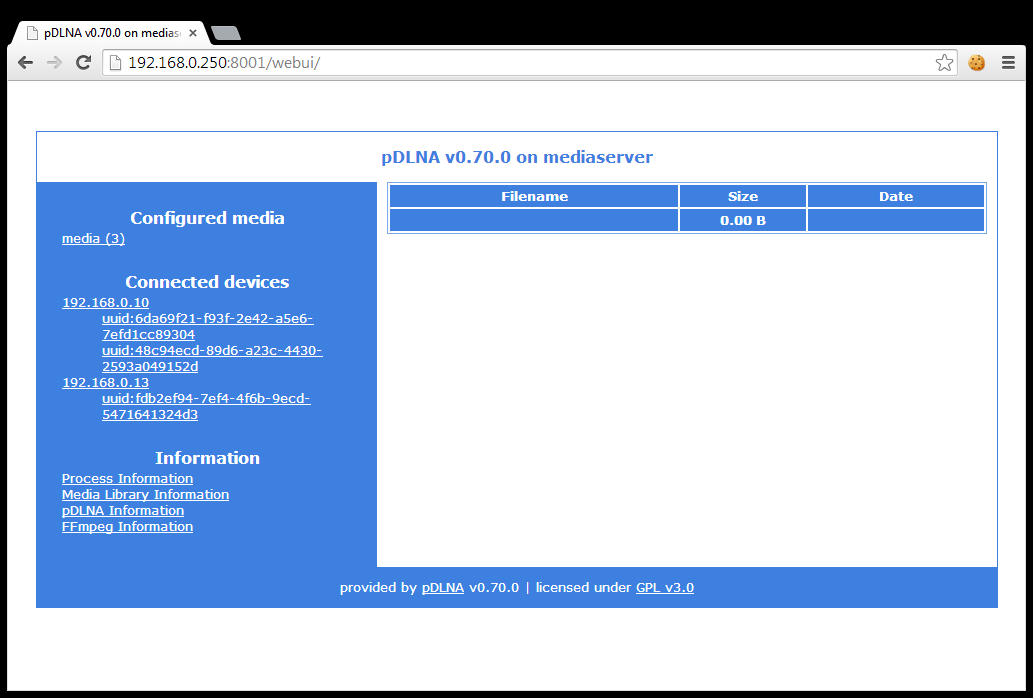
\includegraphics[width=34em]{images/webui_content_landing}
	\label{fig:webgui-landingpage}
	\caption{WebUI: Landing page}
\end{figure}

By clicking (in this case) on the {\em media} directory, the directory tree will be shown as it appears in figure~\ref{fig:webgui-audio}. With an additional click on the {\em audio} directory, the files, which are in this directory will be shown in the content part of the WebUI. The content table, as can be seen, shows the information about the filename, the size and the date of the media file.

\begin{figure}
	\centering
		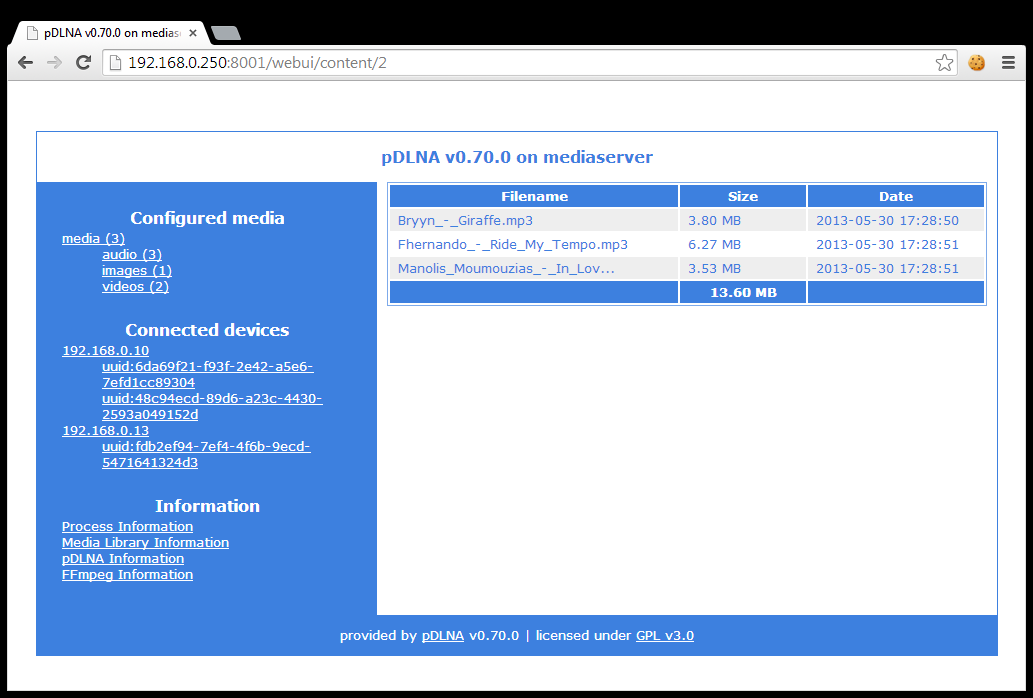
\includegraphics[width=34em]{images/webui_content_audio}
	\label{fig:webgui-audio}
	\caption{WebUI: Directory listing}
\end{figure}

\section{Connected devices}

The second section in the navigation of the WebUI lists all discovered IP addresses, which are part of your network and do interact somehow with the running {\em pDLNA} installation. This includes normal clients, which access the WebUI, other {\em UPnP} devices, {\em DLNA} aware TVs or even other {\em DLNA} media servers.

In the navigation, a list of IP addresses is shown. Additionally, all discovered {\em UPnP} services, which are served by a specifc IP address are also shown in the navigation as subitems.

Figure~\ref{fig:webgui-connecteddevice-ip} shows in the content part the information after clicking on the IP address {\em 192.168.0.130} in the navigation. This information includes the IP address itself, the {\em HTTP UserAgent}, which was used by the device and when communication from the IP address was seen last.

\begin{figure}
	\centering
		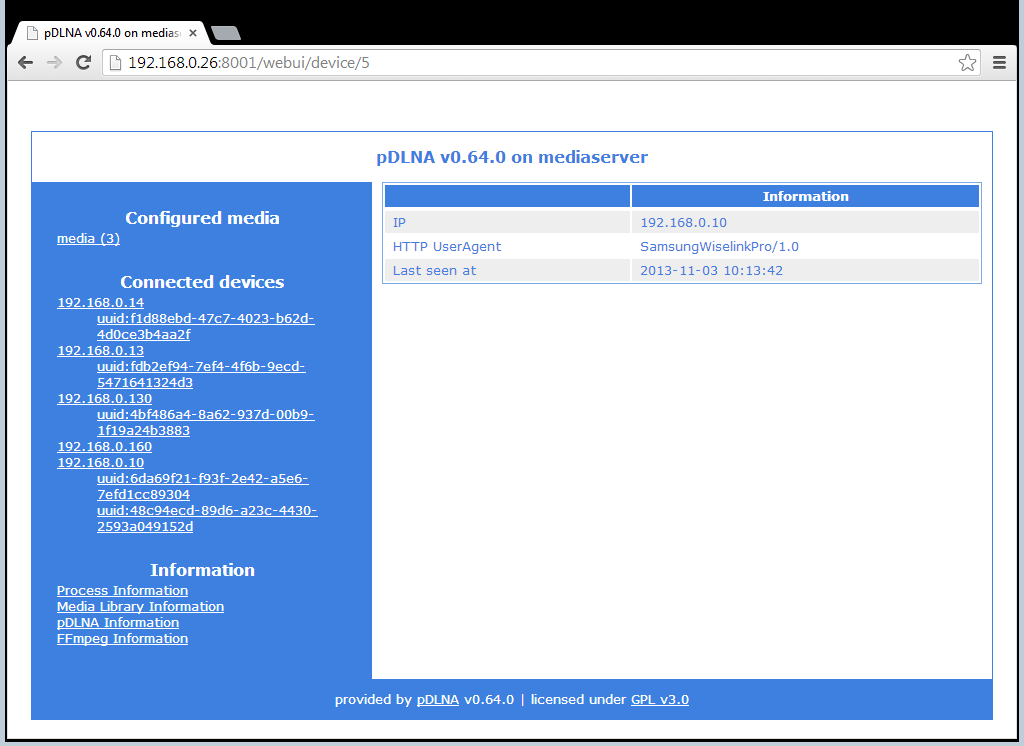
\includegraphics[width=34em]{images/webui_device_ip}
	\label{fig:webgui-connecteddevice-ip}
	\caption{WebUI: Information about a connected device per IP address}
\end{figure}

Figure~\ref{fig:webgui-connecteddevice-service} shows information, including the friendly name, the device type or the device description URL, after clicking on a service UDN.

\begin{figure}
	\centering
		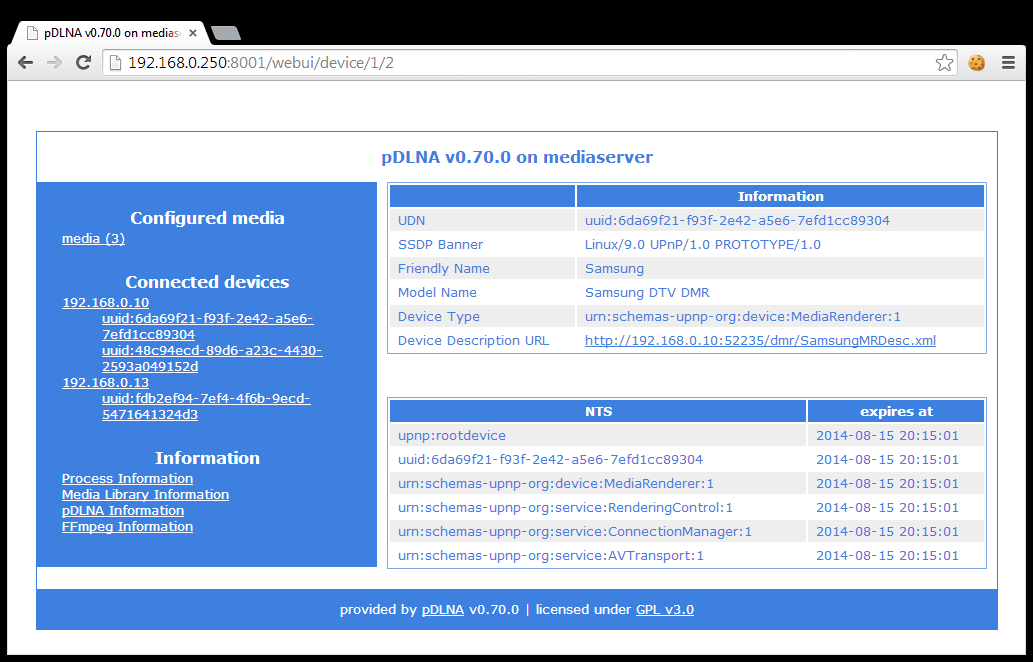
\includegraphics[width=34em]{images/webui_device_ip_service}
	\label{fig:webgui-connecteddevice-service}
	\caption{WebUI: Information about a connected device per service}
\end{figure}

\section{Statistics}

The third section in the navigation includes some statistics about the running{\em pDLNA} installation.

While figure~\ref{fig:webgui-process} shows information about the process itself (including for instance memory and cpu usage), figure~\ref{fig:webgui-library} delivers information about the amount and size of media items included in the media library.

\begin{figure}
	\centering
		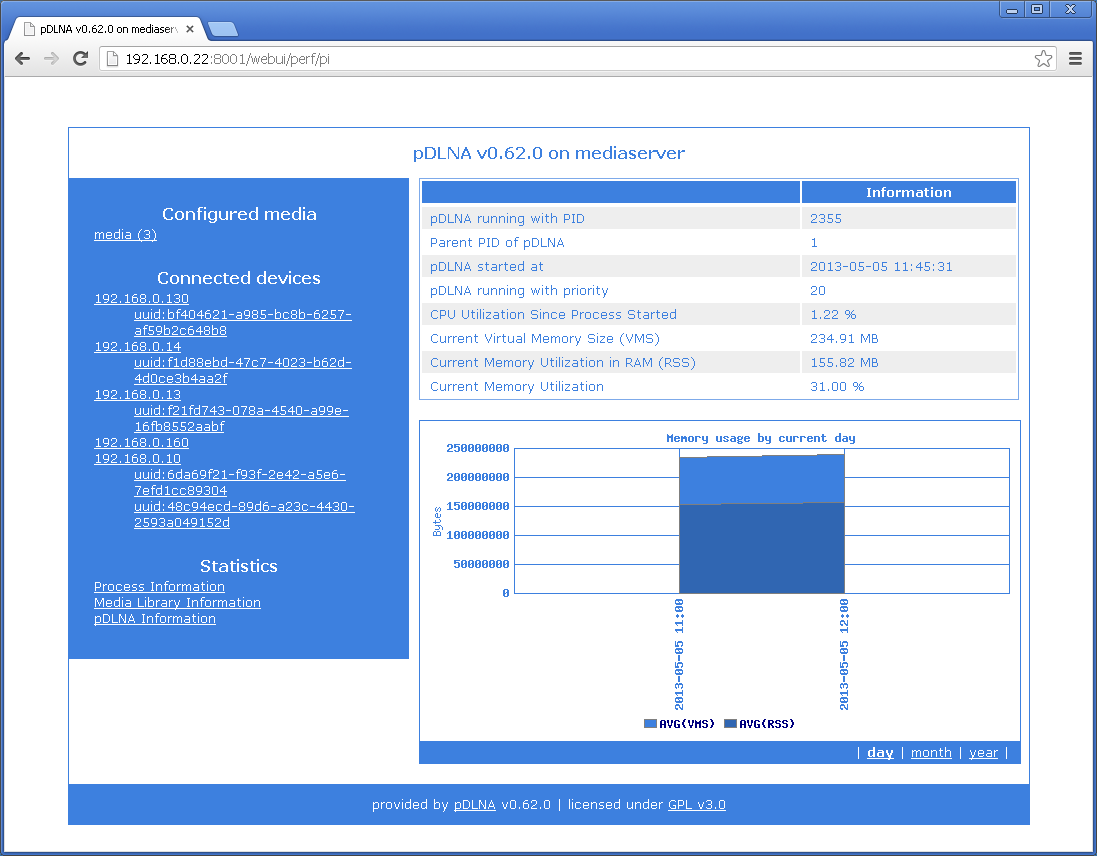
\includegraphics[width=34em]{images/webui_stats_process}
	\label{fig:webgui-process}
	\caption{WebUI: Process Information}
\end{figure}

\begin{figure}
	\centering
		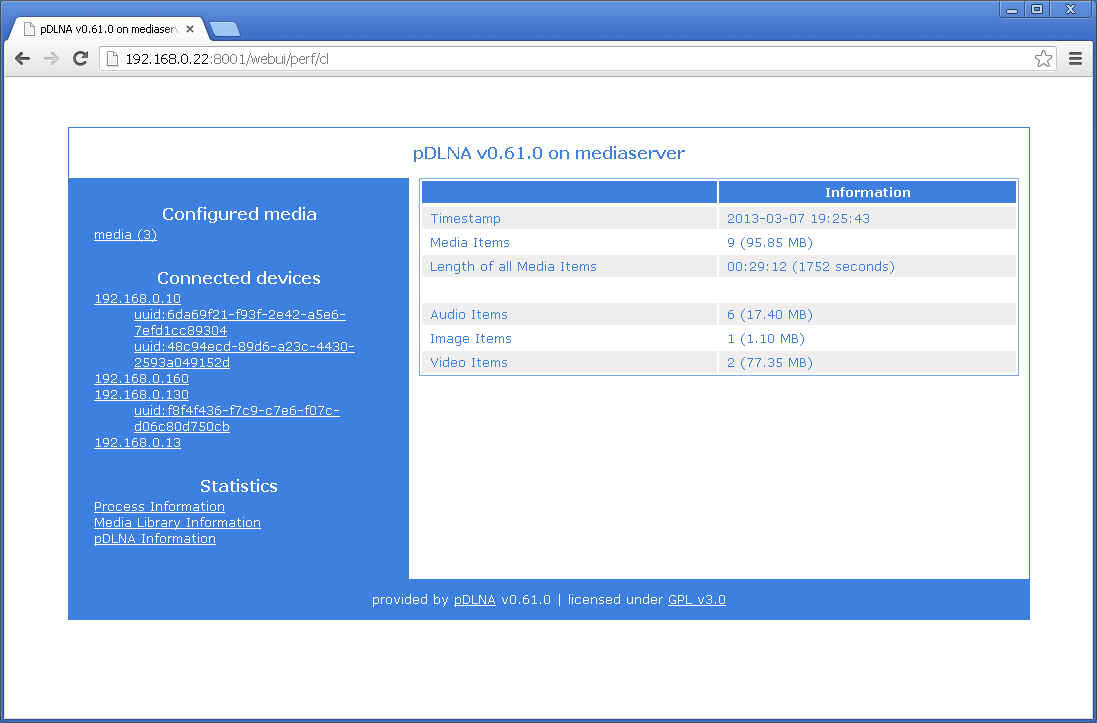
\includegraphics[width=34em]{images/webui_stats_library}
	\label{fig:webgui-library}
	\caption{WebUI: Media Library Information}
\end{figure}

And finally, the following figure~\ref{fig:webgui-pdlna} shows information about the installed {\em pDLNA} version and its release date. You are also able to execute a {\em Check4Updates}, which works as described in section~\ref{config-check4updates}, but shows the result in the WebUI.

\begin{figure}
	\centering
		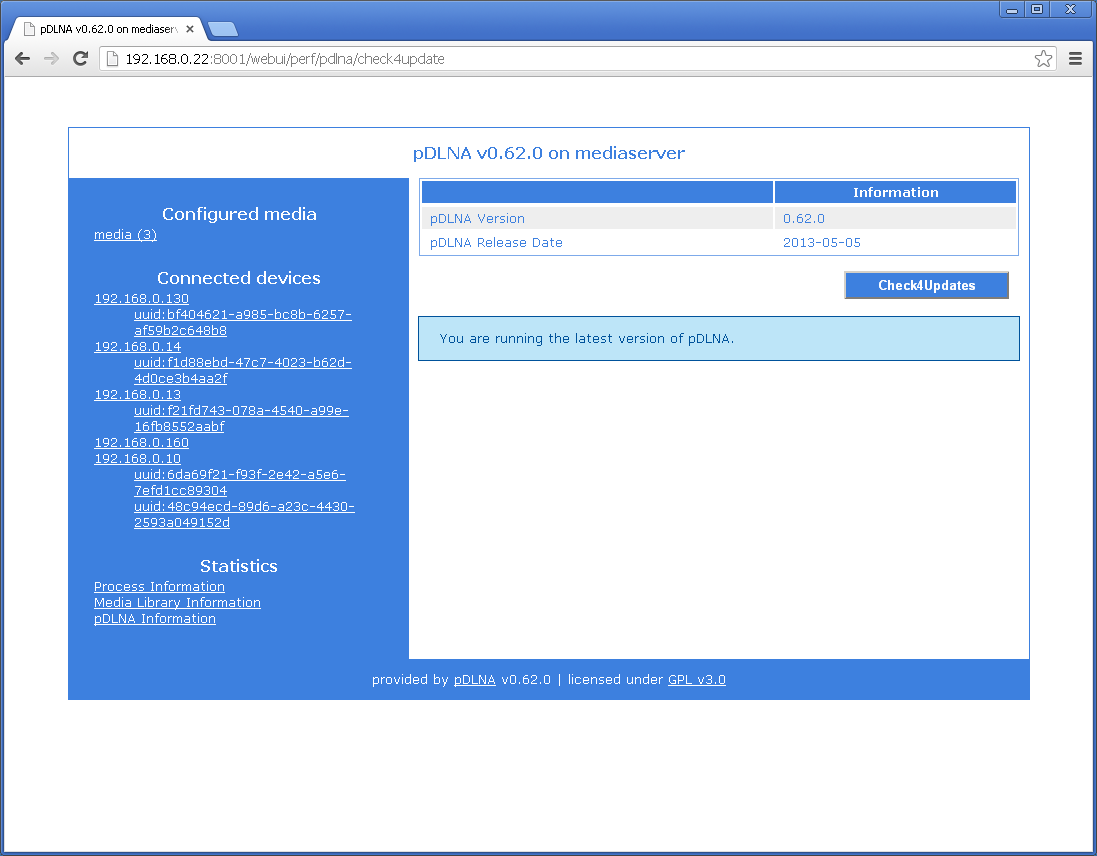
\includegraphics[width=34em]{images/webui_stats_pdlna}
	\label{fig:webgui-pdlna}
	\caption{WebUI: pDLNA Information}
\end{figure}

%
% Preinstalled VMs
%

\chapter{Preinstalled VMware images}
\label{vms}

Since not everybody is willing to install {\em pDLNA} on a system, just to verify if {\em pDLNA} fullfills his needs or just likes to test {\em pDLNA} for the first time, there are some preinstalled {\em VMware} images available to download from the {\em pDLNA} website available under the following URL: \url{www.pdlna.com/cgi-bin/index.pl?menu=vm}

In the case, that somebody does not know {\em VMware}: VMware Player is free for personal use and is available to download via the following URL: \url{www.vmware.com/products/player/overview.html}

You also might be able to convert the available {\em VMware} images and open it with {\em VirtualBox}\footnote{{\em VirtualBox} is an open source virtualization product, which is available on the product website: \url{www.virtualbox.org}.} or any other virtualization product.

\begin{colframeimportantnote}
\textsc{IMPORTANT NOTE:} These preinstalled {\em VMware} images are prepared to have a quick look on {\em pDLNA} and are not designed to be used in a productive environment or for any other purpose.
\end{colframeimportantnote}

While the following section~\ref{vms-general} gives an overview about the general information, like installation of the operating system or the included media files, section~\ref{vms-specifc} describes some per operating system relevant information.

\section{General information}
\label{vms-general}

All the available preinstalled {\em VMware} images are configured the same and do have the following hardware applied:
\begin{itemize}
	\item 512 megabytes of memory
	\item harddisk with 10 gigabytes capacity
	\item one network card which is bridged
\end{itemize}

Afterwards the operating system has been installed, \textbf{english} as language is chosen. Additionally the timezone is set to \textbf{Central European Summer Time (CEST)} and the keyboard layout is set to \textbf{english} too. Finally, if a package management tool is used by the operating system itself, a mirror from \textbf{Austria} is configured. If these settings does not match your needs, please feel free to modify these settings. The following section~\ref{vms-specifc} gives you some short information how to change some of these configurations.

With the installation, the password for the superuser \textbf{root} is set to \textbf{pdlna}. Additionally, another user \textbf{pdlna} with the password \textbf{pdlna} is created. The networkcard is configured to aquire an IP address via {\em DHCP}. Also a {\em SSH} server for remote access and a {\em NTP} server to time synchronization is installed.

Afterwards, all the necessary packages and Perl modules were installed like described int section~\ref{install-prerequisites}. And finally, {\em pDLNA} was installed via a \verb|git clone|, by the user \textbf{pdlna} to the directory \verb|/home/pdlna/pDLNA/|, which is described in section~\ref{install-git}. So the configuration file is stored in \verb|/etc/pdlna.conf| and the initscript to start and stop {\em pDLNA} is stored in \verb|/etc/init.d/rc.pDLNA| or \verb|/etc/rc.d/rc.pDLNA restart|.

\begin{colframeimportantnote}
\textsc{IMPORTANT NOTE:} Every preinstalled {\em VMware} image will not start the {\em pDLNA} installation automatically at startup. So please start {\em pDLNA} by executing \verb|/etc/init.d/rc.pDLNA start| as a superuser.
\end{colframeimportantnote}

Because of installing {\em pDLNA} via \verb|git|, updating the {\em pDLNA} version of an already downloaded {\em VMware} image can be done, by logging in as the user \textbf{pdlna}, changing to the directory \verb|/home/pdlna/pDLNA/| and executing the command \verb|git pull|. And after executing \verb|/etc/init.d/rc.pDLNA restart| or \verb|/etc/rc.d/rc.pDLNA restart| as a superuser, the new version of {\em pDLNA} should be up and running again. This is described in detail in section~\ref{install-unix-git-update}.

\subsection{Included media files}

Each {\em VMware} image comes with the same media files (to test the functionality), which are licensed under the {\em Creative Commons} licence\footnote{\url{www.creativecommons.org}}. In each {\em VMware} image, there is a \verb|DISCLAIMER.txt| file in the directory \verb|/home/pdlna/media/|, which lists the included media files, their source and their exact {\em Creative Commons} licence.

The following list also lists the included media files, their source and their exact {\em Creative Commons} licence:
\begin{itemize}
	\item \verb|/home/pdlna/media/audio/Bryyn_-_Giraffe.mp3|
	\begin{itemize}
		\item Source: \url{www.jamendo.com/de/track/725574/giraffe}
		\item License: \url{creativecommons.org/licenses/by-nc-sa/3.0/}
	\end{itemize}
	\item \verb|/home/pdlna/media/audio/Fhernando_-_Ride_My_Tempo.mp3|
	\begin{itemize}
		\item Source: \url{www.jamendo.com/de/track/944721/ride-my-tem}
		\item License: \url{creativecommons.org/licenses/by-nc-sa/3.0/}
	\end{itemize}
	\item \verb|/home/pdlna/media/audio/Manolis_Moumouzias_-_In_Love.mp3|
	\begin{itemize}
		\item Source: \url{www.jamendo.com/de/track/917546/in-love}
		\item License: \url{creativecommons.org/licenses/by-nc-sa/3.0/}
	\end{itemize}
	\item \verb|/home/pdlna/media/images/Two-toed_sloth_Costa_Rica_-_cropped.jpg|
	\begin{itemize}
		\item Source: \url{upload.wikimedia.org/wikipedia/commons/8/8b/Two-toed_sloth_Costa_Rica_-_cropped.jpg}
		\item License: \url{creativecommons.org/licenses/by/2.5/deed.de}
	\end{itemize}
	\item \verb|/home/pdlna/media/video/episode2.0_xvid.avi|
	\begin{itemize}
		\item Source: \url{archive.org/details/welcometothescene_version2.0_xvid}
		\item License: \url{creativecommons.org/licenses/by-nc-nd/3.0/}
	\end{itemize}
	\item \verb|/home/pdlna/media/video/episode2.0_xvid.mp4|
	\begin{itemize}
		\item Source: \url{archive.org/details/welcometothescene_version2.0_xvid}
		\item License: \url{creativecommons.org/licenses/by-nc-nd/3.0/}
	\end{itemize}
\end{itemize}

The included media files are chosen by random.

\begin{colframeimportantnote}
\textsc{IMPORTANT NOTE:} If you are the copyright owner or an agent thereof and do not want your creation to be distributed like this, please contact me and I will remove your creation.
\end{colframeimportantnote}

\section{Specific Information}
\label{vms-specifc}

The following sections describe some specific settings, which are made to the different preinstalled {\em VMware} images and also describes how to change some of the settings like the timezone or the keyboard layout.

\subsection{CentOS 6}

\begin{colframeimportantnote}
\textsc{IMPORTANT NOTE:} Since \verb|MPlayer| and \verb|FFmpeg| are not part of the package management in CentOS 6, {\em pDLNA} is only able run in {\em LowResourceMode} in this preinstalled {\em VMware} image.
\end{colframeimportantnote}

\subsubsection{Logon customization}

The logon customization, as can be seen in figure~\ref{fig:centos6-loginscreen}, is handeled by the script \verb|/etc/rc.local|, which was modified to call \verb|/usr/local/bin/update-issue.sh|, which updates the \verb|/etc/issue| and \verb|/etc/issue.net| files. The following three lines have also been added to this file, to delete sensitive data on startup:
\begin{colframefile}
\begin{verbatim}
/bin/rm -f /var/log/pdlna.log
/bin/rm -f /tmp/pdlna.db
/bin/rm -f /var/run/pdlna.pid
\end{verbatim}
\end{colframefile}

Additionally, the \verb|OpenSSH| server's configuration file (\verb|/etc/ssh/sshd_config|) has been modified to use the \verb|/etc/issue.net| file as a banner:
\begin{colframefile}
\begin{verbatim}
Banner /etc/issue.net
\end{verbatim}
\end{colframefile}

The \verb|/usr/local/bin/update-issue.sh| script can also be found on GitHub (\url{github.com/geuma/pDLNA-utils/blob/master/preinstalled-VMs/CentOS6/update-issue.sh}).

\begin{figure}
	\centering
		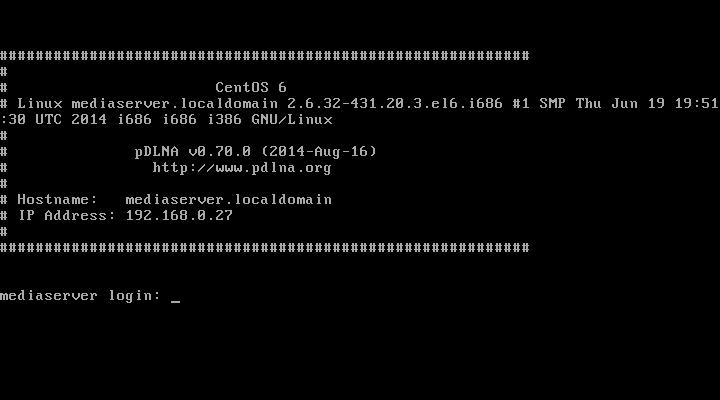
\includegraphics[width=34em]{images/vm_centos6_loginscreen}
	\label{fig:centos6-loginscreen}
	\caption{Boot-up screen of preinstalled CentOS 6 VMware image}
\end{figure}

\subsubsection{Changing the timezone}

In CentOS 6, all the available timezones are stored in the directory \verb|/usr/share/zoneinfo/|. Because of this, changing the timezone can be done via modifying the sysmlink for \verb|/etc/localtime| to the corresponding timezone file. An example is listed in the following snippet:

\begin{colframecmd}
\begin{verbatim}
pdlna@mediaserver:~$ sudo ln -sf /usr/share/zoneinfo/EST
  /etc/localtime
\end{verbatim}
\end{colframecmd}

\subsubsection{Changing the keyboard layout}

In CentOS 6, all the available keyboard layouts are stored in the directory \verb|/lib/kbd/keymaps/i386|. Changing the keyboard layout can be done via modifying the \verb|KEYTABLE| key in the file \verb|/etc/sysconfig/keyboard| by opening the file with your favourite file editor:

\begin{colframecmd}
\begin{verbatim}
pdlna@mediaserver:~$ sudo vi /etc/sysconfig/keyboard
\end{verbatim}
\end{colframecmd}

Additional documentation can be found here: \url{www.centos.org/docs/5/html/5.1/Deployment_Guide/s2-sysconfig-kybd.html}

\subsection{Debian GNU/Linux 7}

\subsubsection{Logon customization}

The logon customization, as can be seen in figure~\ref{fig:debian7-loginscreen}, is handeled by the script \verb|/etc/rc.local|, which was modified to call \verb|/usr/local/bin/update-issue.sh|, which updates the \verb|/etc/issue| and \verb|/etc/issue.net| files. The following three lines have also been added to this file, to delete sensitive data on startup:
\begin{colframefile}
\begin{verbatim}
/bin/rm -f /var/log/pdlna.log
/bin/rm -f /tmp/pdlna.db
/bin/rm -f /var/run/pdlna.pid
\end{verbatim}
\end{colframefile}

Additionally, the \verb|OpenSSH| server's configuration file (\verb|/etc/ssh/sshd_config|) has been modified to use the \verb|/etc/issue.net| file as a banner:
\begin{colframefile}
\begin{verbatim}
Banner /etc/issue.net
\end{verbatim}
\end{colframefile}

The \verb|/usr/local/bin/update-issue.sh| script can also be found on GitHub (\url{github.com/geuma/pDLNA-utils/blob/master/preinstalled-VMs/Debian7/update-issue.sh}).

\begin{figure}
	\centering
		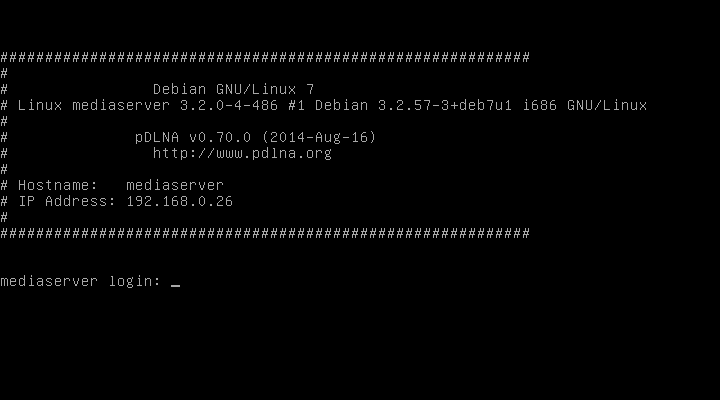
\includegraphics[width=34em]{images/vm_debian7_loginscreen}
	\label{fig:debian7-loginscreen}
	\caption{Boot-up screen of preinstalled Debian 7 VMware image}
\end{figure}

\subsubsection{Changing the timezone}

Changing the timezone in Debian GNU/Linux 7 can be done by executing the following command as a superuser and use its wizard to configure the correct timezone.

\begin{colframecmd}
\begin{verbatim}
pdlna@mediaserver:~$ sudo dpkg-reconfigure tzdata
\end{verbatim}
\end{colframecmd}

\subsubsection{Changing the keyboard layout}

Changing the keyboard layout is as easy as changing the timezone. Just execute the following command as a superuser and use its wizard to configure the correct keyboard layout.

\begin{colframecmd}
\begin{verbatim}
pdlna@mediaserver:~$ sudo dpkg-reconfigure keyboard-configuration
\end{verbatim}
\end{colframecmd}

\subsection{FreeBSD 9}

\subsubsection{Logon customization}

The logon customization, as can be seen in figure~\ref{fig:freebsd9-loginscreen}, is handeled by the script \verb|/etc/rc.local|, which was created to call \verb|/usr/local/bin/update-issue.sh|, which updates the \verb|/etc/issue| and \verb|/etc/issue.net| files and delete sensitive data. The script \verb|/etc/rc.local| has been created with the following content and the executable bit has been set. By default, FreeBSD 9 executes this script at startup via \verb|/etc/rc.d/local|.
\begin{colframefile}
\begin{verbatim}
#!/bin/sh

/usr/local/bin/update-issue.sh
/bin/rm -f /var/log/pdlna.log
/bin/rm -f /tmp/pdlna.db
/bin/rm -f /var/run/pdlna.pid
\end{verbatim}
\end{colframefile}

Since the configuration file \verb|/etc/gettytab| is already configured to use the \verb|/etc/issue| file as a banner, no configuration to \verb|getty| was needed.

Additionally, the \verb|OpenSSH| server's configuration file (\verb|/etc/ssh/sshd_config|) has been modified to use the \verb|/etc/issue.net| file as a banner:
\begin{colframefile}
\begin{verbatim}
Banner /etc/issue.net
\end{verbatim}
\end{colframefile}

The \verb|/usr/local/bin/update-issue.sh| script can also be found on GitHub (\url{github.com/geuma/pDLNA-utils/blob/master/preinstalled-VMs/FreeBSD9/update-issue.sh}).

\begin{figure}
	\centering
		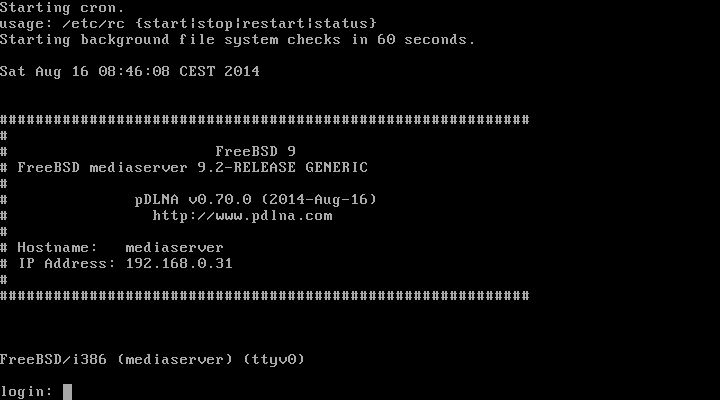
\includegraphics[width=34em]{images/vm_freebsd9_loginscreen}
	\label{fig:freebsd9-loginscreen}
	\caption{Boot-up screen of preinstalled FreeBSD 9 VMware image}
\end{figure}

\subsubsection{Changing the timezone}

In FreeBSD 9, all the available timezones are stored in the directory \verb|/usr/share/zoneinfo|. Because of this, changing the timezone can be done via copying the corresponding timezone file to \verb|/etc/localtime|. An example is listed in the following snippet:

\begin{colframecmd}
\begin{verbatim}
[pdlna@mediaserver ~]$ sudo copy /usr/share/zoneinfo/EST
  /etc/localtime
\end{verbatim}
\end{colframecmd}

\subsubsection{Changing the keyboard layout}

Changing the keyboard layout is as easy as changing the timezone. Just execute the following command as a superuser and use its menu to configure the correct keyboard layout.

\begin{colframecmd}
\begin{verbatim}
[pdlna@mediaserver ~]$ sudo kbdmap
\end{verbatim}
\end{colframecmd}

If you would like to change the keyboard layout in a persistent way, modify the file \verb|/etc/rc.conf|.

%
% Troubleshooting
%

\chapter{Debugging and reporting problems}
\label{troubleshooting}

This is not (yet) a real troubleshooting guide to {\em pDLNA}. Currently it is more a small handbook to do some general debugging and how to gather some necessary information on a running Linux operating system. You are also able to forward this information to me.

\section{Debugging}

When starting {\em pDLNA}, the process will parse the configuration file\footnote{Please see chapter~\ref{config} for more details.} and will not start until everything is configured correctly. In some cases {\em pDLNA} might not be able to determine the correct {\em ListenInterface}, where you need to configure those information by hand. The following command starts {\em pDLNA}.
\begin{colframecmd}
\begin{verbatim}
pdlna@mediaserver:~$ sudo /etc/init.d/rc.pDLNA start
\end{verbatim}
\end{colframecmd}

Once {\em pDLNA} is running successfully, you are able to verify this by running the following two commands. The first one checks all the running processes for the {\em pDLNA} process, while the second one prints out the stored PID. If both PID match each other, everything should be fine.

\begin{colframecmd}
\begin{verbatim}
pdlna@mediaserver:~$ sudo ps -ef | grep pDLNA
root     13162     1  3 09:18 pts/2    00:00:50
  /usr/bin/perl ./pDLNA.pl -f /etc/pdlna.conf
\end{verbatim}
\end{colframecmd}

\begin{colframecmd}
\begin{verbatim}
pdlna@mediaserver:~$ sudo cat /var/run/pdlna.pid
13162
\end{verbatim}
\end{colframecmd}

The following listings are based on the network configuration listed in~\ref{confignetwork}. So, the next step to identify a lowlevel network problem of {\em pDLNA} will be to check if {\em pDLNA} is listening to the two necessary network ports. On the one hand, there is \textbf{port 1900 UDP} needed for the {\em SSDP} communication and \textbf{port 8001 TCP}\footnote{Please ensure that this port can be changed in the configuration file and {\em 8001} is the default one.} for the {\em DLNA} communication via HTTP. The following command checks the network statistics and filters for the lines including the PID of the running {\em pDLNA} installation.
\begin{colframecmd}
\begin{verbatim}
pdlna@mediaserver:~$ sudo netstat -taunp | grep 13162
Active Internet connections (servers and established)
Proto Recv-Q Send-Q Local Address
 Foreign Address         State       PID/Program name
tcp        0      0 192.168.145.139:8001
 0.0.0.0:*               LISTEN      13162/perl
udp        0      0 192.168.145.139:37302
 239.255.255.250:1900    ESTABLISHED 13162/perl
udp    53368      0 0.0.0.0:1900
 0.0.0.0:*                           13162/perl
\end{verbatim}
\end{colframecmd}
If your network statistics output shows, that {\em pDLNA} is correctly listening to \textbf{port 1900 UDP} and the configured {\em HTTPPort}, the network communication should be working.

\begin{colframeimportantnote}
\textsc{IMPORTANT NOTE:} {\em AllowedClients} is configured to the local subnet by default.
\end{colframeimportantnote}

\begin{colframeimportantnote}
\textsc{IMPORTANT NOTE:} Please also check your firewall configuration.
\end{colframeimportantnote}

As a simple test you can visit the WebUI (see chapter~\ref{webui}), which can be accessed by the following URL: \verb|http://ListenIPAddress:HTTPPort/webui/|. If you are receiving an {\em HTTP Error Code 403}, your host is not configured as an {\em AllowedClients}. If your Browser is running in a {\em timeout}, there might be a problem with your configuration.

After checking the general process and network information, the next step is about increasing the {\em LogLevel} and configuring the necessary {\em LogCategory} from table~\ref{tab:AvailableLogCategoryparams}. At first you need to configure {\em LogLevel} to the highest {\em LogLevel} available in table~\ref{tab:AvailableLogLevelparams} for the most detailed log messages.

\subsection{My device is not able to discover {\em pDLNA}}

If your {\em DLNA} capable device is not able to discover {\em pDLNA}, please set the configuration parameter {\em LogCategory} to \verb|discovery, httpgeneric| and restart {\em pDLNA}. Additionally you are able to do a packet capture with the following command:
\begin{colframecmd}
\begin{verbatim}
pdlna@mediaserver:~$ sudo tcpdump -i ListenInterface \
 -s 1500 -w capture_full.pcap
\end{verbatim}
\end{colframecmd}
Please ensure to fill in the configured {\em ListenInterface}.

\subsection{My media directories are not read correctly}

In the case, that {\em pDLNA} was not able to read in your shared directories correctly, enable the {\em LogCategory} \verb|library| in the configuration file and restart the installed version of {\em pDLNA}. An easy way to navigate quickly through the media library and check for problems is by using the WebUI (see chapter~\ref{webui}).

For a detailed look on the structure and contents of the media library, check your database.

\subsection{My device is not able to list the directories/items shared by {\em pDLNA}}

If browsing the shared media directories is not working properly by your {\em DLNA} aware devices, configure the {\em LogCategory} to \verb|httpgeneric, httpdir|, restart {\em pDLNA} and do a packet capture with the following command:
\begin{colframecmd}
\begin{verbatim}
pdlna@mediaserver:~$ sudo tcpdump -p HTTPPort -s \
 1500 -w capture_http.pcap
\end{verbatim}
\end{colframecmd}
Please ensure to fill in the configured {\em HTTPPort} (by default set to \verb|8001|).

For a detailed look on the structure and contents of the media library, check your database.

\subsection{{\em pDLNA} is not able to stream media items to my device}

In any case, that streaming of videos, music or images is not working properly, please set the {\em LogCategory} parameter to \verb|httpgeneric, httpstream|, restart {\em pDLNA} and start a packet capture with the following command:
\begin{colframecmd}
\begin{verbatim}
pdlna@mediaserver:~$ sudo tcpdump -p HTTPPort \
 -s 1500 -w capture_http.pcap
\end{verbatim}
\end{colframecmd}
Please ensure to fill in the configured {\em HTTPPort} (by default set to \verb|8001|).

\section{Reporting problems}

If you are not able to fix the problem or just want me to take a closer look, please supply all mentioned information, like network statistics, packet captures, logs and so on.

In case of having a {\em DLNA} aware device, which is not working properly with {\em pDLNA} please supply a full packet capture, including the whole {\em SSDP} and {\em DLNA} packets of this specific device communicating with another digital media server (which is working properly). In this case I might be able to deternmine the differences and supply a new version of {\em pDLNA} which is supporting this device.

%
% KNOWN ISSUES
%

\chapter{Known Issues}
\label{knownissues}

%Currently there are no known issues. If you have found an issue while running {\em pDLNA}, please report the issue via mail or via \url{https://github.com/geuma/pDLNA/issues}.

\section{FreeBSD: initscript unable to completely shut down pDLNA}

\subsection{Description}

On FreeBSD, there seems to be a problem shutting down {\em pDLNA} via the included initscript\footnote{\url{https://github.com/geuma/pDLNA/issues/20}}. After stopping and starting {\em pDLNA}, the following error message will occur:
\begin{colframecmd}
\begin{verbatim}
[root@mediaserver ~]# /etc/rc.d/rc.pDLNA start
Starting pDLNA ...
[root@mediaserver ~]# /etc/rc.d/rc.pDLNA restart
Starting pDLNA ...
[root@mediaserver ~]# Cannot bind to Multicast socket:
 Address already in use
Going to terminate pDLNA/v0.63.0 on freebsd/9.0-release
 with FriendlyName 'pDLNA v0.63.0 on mediaserver' ...
\end{verbatim}
\end{colframecmd}

\subsection{Workaround}

Since there is no fix for this issue today, this problem can be handled by a workaround. Get the process ID of the still running {\em pDLNA} process, kill it, remove the PID file (if any) and use the initscript afterwards again to start {\em pDLNA}:
\begin{colframecmd}
\begin{verbatim}
[root@mediaserver ~]# ps | grep pDLNA
2327   0  I    0:22.46 /usr/bin/perl ./pDLNA.pl -f /etc/pdlna.conf
2651   0  R+   0:00.01 grep pDLNA
[root@mediaserver ~]# kill -9 2327
[root@mediaserver ~]# rm /var/run/pdlna.pid
[root@mediaserver ~]# /etc/rc.d/rc.pDLNA start
Starting pDLNA ...
\end{verbatim}
\end{colframecmd}

%
% FIXED ISSUES
%

\chapter{Fixed Issues}
\label{fixedissues}

\section{Use of uninitialized value \$request\_line in string ne at /PDLNA/HTTPServer.pm line xxx.}

\begin{colframeimportantnote}
\textsc{IMPORTANT NOTE:} This issue has been fixed with {\em pDLNA} in version 0.62.0.
\end{colframeimportantnote}

\subsection{Describtion}

Apparently {\em pDLNA} sometimes starts to print, for unknown reasons, the following warning message to \verb|STDOUT| infinitely\footnote{\url{github.com/geuma/pDLNA/issues/13}}:
\begin{colframecmd}
\begin{verbatim}
Use of uninitialized value $request_line in string ne at
  /PDLNA/HTTPServer.pm line xxx.
\end{verbatim}
\end{colframecmd}

\subsection{Workaround}

Since, this message is only a warning message, it does not affect the functionality of {\em pDLNA}. But actually, it increases the system load. A restart of {\em pDLNA} will fix the problem temporarily, but the issue might take place again.

\section{AllowedClients auto detection on FreeBSD is defect}

\begin{colframeimportantnote}
\textsc{IMPORTANT NOTE:} This issue has been fixed with {\em pDLNA} in version 0.61.0.
\end{colframeimportantnote}

\subsection{Describtion}

Apparently {\em pDLNA} dies with the following error message on {\em FreeBSD} if {\em AllowedClients} auto detection is enabled\footnote{\url{github.com/geuma/pDLNA/issues/4}}:
\begin{colframecmd}
\begin{verbatim}
AllowedClients(ip_address_sv) at PDLNA/Config.pm line xxx.
\end{verbatim}
\end{colframecmd}
This seems to be a problem with the usage of \verb|AllowedClients(ip_address_sv)| on {\em FreeBSD}.

\subsection{Workaround}

As a workaround you are able to define the {\em AllowedCLients} configuration parameter in the conifguration file. For detailed information see section~\ref{confallowedclients}.

\end{document}
